\chapter{胰腺}

\section{检查方法}

\subsection{检查前准备}

检查前要求患者空腹4~6小时。检查前30分钟口服2%泛影葡胺溶液500~700ml,以充盈近段空肠;扫描前即刻再服300~500ml同样液体,以充盈胃十二指肠。扫描前15~20分钟亦可肌注山莨菪碱20mg,以减少胃肠蠕动。充盈胃肠道亦可用清水代替。

\subsection{常用检查方法}

1.常规平扫:从膈顶开始按上腹部常规层厚和间隔(如10mm)做连续扫描,直至胰腺全部显示为止,胰腺范围约在T\textsubscript{11}
至L\textsubscript{2} 水平。

2.动态增强扫描:包括动床式和同层面两种方式,以前者常用。一般采用薄层、团注造影剂法,以流率2~4ml/s注入造影剂80~100ml(总量按1.5~2ml/kg计算)。开始注射造影剂后15~20秒开始扫描,层厚及间距3~5mm。

3.螺旋CT增强扫描:国内有研究表明,高剂量可提高胰腺的增强效果,可采用1.5ml/kg总剂量,以2.5~3ml/s流率注入造影剂。行动脉期(18~25秒)、实质期(40秒)和门静脉期(65~70秒)扫描。层厚3~5mm,螺距1~1.4。国内有学者主张仅行实质期和门静脉期双期扫描即可。

此外,螺旋CT尤其是多层螺旋CT的应用,也促进了胰腺灌注成像的应用。国外有研究表明胰腺的正常灌注量为1.25ml/(min·ml),SD
0.16。

\section{正常解剖、CT表现和变异}

\subsection{毗邻关系和形态}

胰腺位于腹膜后腔横过第1~2腰椎前方,其右侧嵌于十二指肠降部与水平部所形成的凹陷内,左侧端伸达脾门。前面被构成网膜囊后壁的后腹膜所覆盖,再向前即为网膜囊下隐窝和胃后壁,后面为腹主动脉、下腔静脉、双侧肾静脉及左肾上腺、腹腔神经丛、胸导管起始端等结构。

胰腺形态略呈三棱形,且狭长。边缘可很光整,也可为规则的锯齿状或轻微分叶。可分为4部分:①头部;②颈部;③体部;④尾部。此外,常将胰头部下方的三角形或楔形钩突称为钩突部。主胰管起自胰尾部,横贯胰腺全长;副胰管位于主胰管的上前方,大多与主胰管相通,不相通者占20%~30%。

\subsection{正常胰腺的CT表现}

胰腺在脾动脉下方、脾静脉前方,走向呈斜行、横形、S形和马蹄形,故横断面扫描形态各异。

1.胰头部:横断面近圆形,位于中线右侧。前方为胃窦,右侧为十二指肠降段,后方为下腔静脉。胰头向下伸展的钩突呈三角形或楔形,尖向左,边缘平直。钩突前方有1对血管即肠系膜上动脉、静脉(动脉在后、静脉在前),钩突右侧是十二指肠降段,下方为十二指肠水平段。

2.颈部:是连接头、体的狭窄扁薄部分,长2~2.5cm。胰头和颈以肠系膜上静脉右缘为界,胰颈位于肠系膜上静脉的前方。

3.体部:位于中线及偏左部分,后有腹腔动脉或肠系膜上动脉。

4.尾部:体、尾无明显的分界线,一般认为左肾前方的部分为尾部。

\subsection{胰腺的大小和测量}

国内有学者统计,头、颈、体和尾的最大径分别为32mm、18.42mm、24.59mm和23.83mm。胰腺大小、密度与年龄呈负相关,儿童较成人大。老年人的胰腺实质因萎缩比中年人小,而主胰管却随年龄的增大而渐宽,但一般直径不超过3mm。

测量大小时,必须注意:①区别紧贴胰体后方走行的脾静脉,不要误为胰腺边缘。②估计胰腺大小的临床意义时,应十分重视胰腺外形。从胰头至胰尾,正常胰腺呈自然曲线,平滑而连续。如突然改变则为异常;如局限性隆起,即使其测量值在正常范围内,也应视为异常。③胰腺退行性变表现为体积的缩小和胰腺的脂肪浸润。60岁以上老人胰腺逐渐萎缩,边缘分叶,切迹深>2mm。④注意勿将脾静脉与胰腺之间的脂肪间隙误为胰管。⑤在脊柱侧弯的病人,胰腺可扭曲变形,勿误为增大。此外,勿将十二指肠降部憩室内充满物质,以及胰头后方的肿大淋巴结误为胰头增大。

\subsection{胰腺的密度}

正常胰腺的密度均匀或欠均匀,与胰腺间质中脂肪含量有关,CT值低于肝脏,与血管和脾脏相近,平扫CT值为30~50Hu,一般增强后CT值增至100~150Hu左右。

\subsection{胰腺的常见变异}

1.分离胰腺:最常见。系大体完整的胰腺内存在两套完全分离、互不相连的胰腺导管系统,是急性胰腺炎重要诱因。薄层CT扫描可发现单独存在的腹胰导管,有时还可直接显示由薄层脂肪分隔开的腹胰部和背胰部。

2.右位胰腺:见于内脏反位者,胰腺大部分位于右侧。

3.分叉胰腺:①由于胰发育过程中胰尾部分叉,形成两部分胰尾;②也可由于肠系膜上动脉或胃网膜左动脉压迫而使胰尾分叉。

4.环状胰腺:胰腺呈环状包绕十二指肠降部,有完全型和不完全型两种。

5.异位胰腺:又称迷走胰腺或副胰,是一种与胰腺本身无丝毫连接的异位生长的胰腺组织。常呈小块状生长,大者直径可达7cm,小者仅0.5cm,一般直径在1~4cm。

此外,还可见短小胰腺、胰腺发育不良等。

\subsection{胰腺异常的CT征象}

胰腺异常的CT表现主要有以下几方面:

1.胰腺增大:为局限性或弥漫性,常因肿瘤或急性胰腺炎引起。

2.胰腺萎缩:除老年人胰腺萎缩外,儿童及成人常因囊性纤维化或慢性胰腺炎引起胰腺实质形成瘢痕而致体积缩小。囊性纤维化还可见实质脂肪浸润、密度减低、胰管扩张、多发大小不等的囊肿形成及微小钙化等,与慢性胰腺炎类似。此外,萎缩还可见于老龄缺血、慢性蛋白质缺乏症、胰管梗阻等。

3.囊样病变:可为炎性、肿瘤性和先天性。

4.脂肪替代:①类固醇治疗、库欣氏综合征或肥胖者,以及老年人引起的脂肪浸润一般较轻。②囊性纤维化呈慢性改变,除脂肪浸润外,还有胰腺萎缩等表现。③胰、血液和骨(Schwachman-Diamond)综合征是干骺端软骨发育不全伴消化道吸收不良和中性粒细胞下降的一组疾病。胰腺完全性的脂肪浸润,初期腺体增大、后期正常或变小,无钙化、囊性改变。④其他伴有脂肪替代的病变还有糖尿病、慢性胰腺炎、酒精性肝炎等。

总之,胰腺被脂肪替代相当常见,这种表现最常见于肥胖和老化。CT表现为实性软组织被混杂的脂肪分隔。更典型的病例中,脂肪已成为胰腺的主要组织成分,特别是老年人可伴有明显的胰腺萎缩。脂肪替代在胰腺的分布可均匀或不均匀。胰头前部容易被脂肪替代,而其后部和胆总管周围脂肪浸润较轻。不均匀的脂肪浸润应与小的胰腺病变相鉴别。

5.创伤性损害。

6.先天发育异常:胰腺分离、环形胰腺、先天性短胰腺、胰腺发育不良和胰腺组织移位等。

此外,国内文献还将胰腺间质脂肪浸润、胰腺萎缩、“休克”胰腺统称为胰腺退化性改变。“休克”胰腺表现为实质内灶性或广泛性的出血灶,但灶周无炎性反应,可能与休克和缺氧有关。常出现在临终前,故又称为“濒死”性胰腺。

\section{胰腺炎症}

\subsection{急性胰腺炎}

急性胰腺炎为最常见的胰腺疾病,也是常见的急腹症之一。

\textbf{【病因】}
①胆源性:在国内半数以上伴胆管疾病如结石、炎症和狭窄等。由于壶腹部梗阻,胆汁返流,胰液外溢导致胰腺无菌性炎症;胆盐激活脂肪酶导致脂肪坏死。②酒精性:酗酒和饱餐后引起胃肠道充血水肿、十二指肠乳头括约肌痉挛,胆汁和胰液返流,同时胰液分泌增加等导致胰腺炎。③十二指肠梗阻、ERCP术后、胃肠和胆道术后及腹部创伤。④感染性:如腮腺炎、病毒性肝炎、内毒素和外毒素作用等。⑤药物性和代谢性:后者如高血脂症、高血钙症。⑥特发性:即原因不明。

\textbf{【病理】}
①单纯水肿型(轻型):又称为急性间质性胰腺炎,多见。主要表现为胰腺间质性水种及胰腺周围坏死,没有胰腺实质的坏死。此型可演变为出血坏死型。②出血坏死型(重型):约占10%~20%。表现为胰周及胰腺广泛的脂肪组织坏死,胰腺实质的坏死及出血可以局限或弥漫。胰腺坏死是由于胆囊收缩素-促胰酶素高于正常,促使胆囊收缩及胰液大量分泌,使胰腺组织自身发生消化作用,急性胰腺炎含胰酶的液体渗出物累及胰腺间质、胰周围间隙脂肪组织。但两型并无截然分界线,且也并非完全是一个病症的两个发展阶段。CT也难以做出明确诊断。

\textbf{【临床表现】}
多见于成年人,起病急骤。主要症状有:①上腹部疼痛,通常为持续性,程度剧烈,常放射到胸背部;②发热及白细胞计数升高;③恶心、呕吐等胃肠道症状;④重者有低血压和休克;⑤腹膜炎体征;⑥其他如黄疸、多器官功能衰竭和各种并发症;⑦化验除白细胞升高外,多伴有血和尿淀粉酶及胰蛋白酶升高。

\textbf{【CT表现】}

1.急性单纯水肿型

本型的诊断主要基于其临床表现及生化检查。约10%~20%的病例CT无阳性发现。

CT主要表现为胰腺增大,通常为整个增大,也可只表现为胰头和(或)胰尾局限性增大。这类表现约占48%。另外,最常见的表现为胰周界限不清晰,实质密度均匀或不均匀,肾周筋膜增厚等。偶尔可见胰腺内或周围少量积液。

应该指出,多数学者认为左肾前筋膜(吉氏筋膜)增厚是胰腺炎的重要标志,尤其是胰腺自身改变不明显时,但左肾前筋膜亦可见于其他腹膜后疾病如肾癌等。该筋膜正常厚约1~2mm,如局限性增厚或均匀增厚>2~3mm为异常。

2.急性出血坏死型

CT表现为:①胰腺增大:常有明显增大,且为弥漫性;胰腺体积增大与临床严重程度一致。②出血和坏死:实质出血平扫时可见胰腺内局灶性CT值增高,实质坏死则表现为增强扫描近囊样的未强化区。国外有学者认为,一个局限的或弥漫的,边界清楚,直径>3cm或者胰腺区30%以上的未强化实质区是CT诊断坏死的一个可靠征象;如胰腺坏死区小时特异性仅占50%。坏死区域累及整个胰腺呈一个“袋状”表现,并伴有可强化的包膜。③感染性坏死:坏死的胰腺实质是感染和脓肿形成的良好基础,其感染性坏死有导致心血管、肾、肝、肺部并发症的危险。急性胰腺炎胰腺组织的感染率为7%~12%,而坏死性胰腺炎感染率为30%~70%。但胰腺坏死是否继发感染需由穿刺针吸活检证实。④胰周改变:其胰周改变较单纯型明显,表现为脂肪坏死和积液。与单纯水肿型胰腺炎一样,液体最常积聚于小网膜囊、左肾旁间隙和横结肠系膜处(图\ref{fig13-1}),只是坏死型渗出液为大量(超过胰腺表面积),而水肿型为少量(小于胰腺表面积)。

\begin{figure}[!htbp]
 \centering
 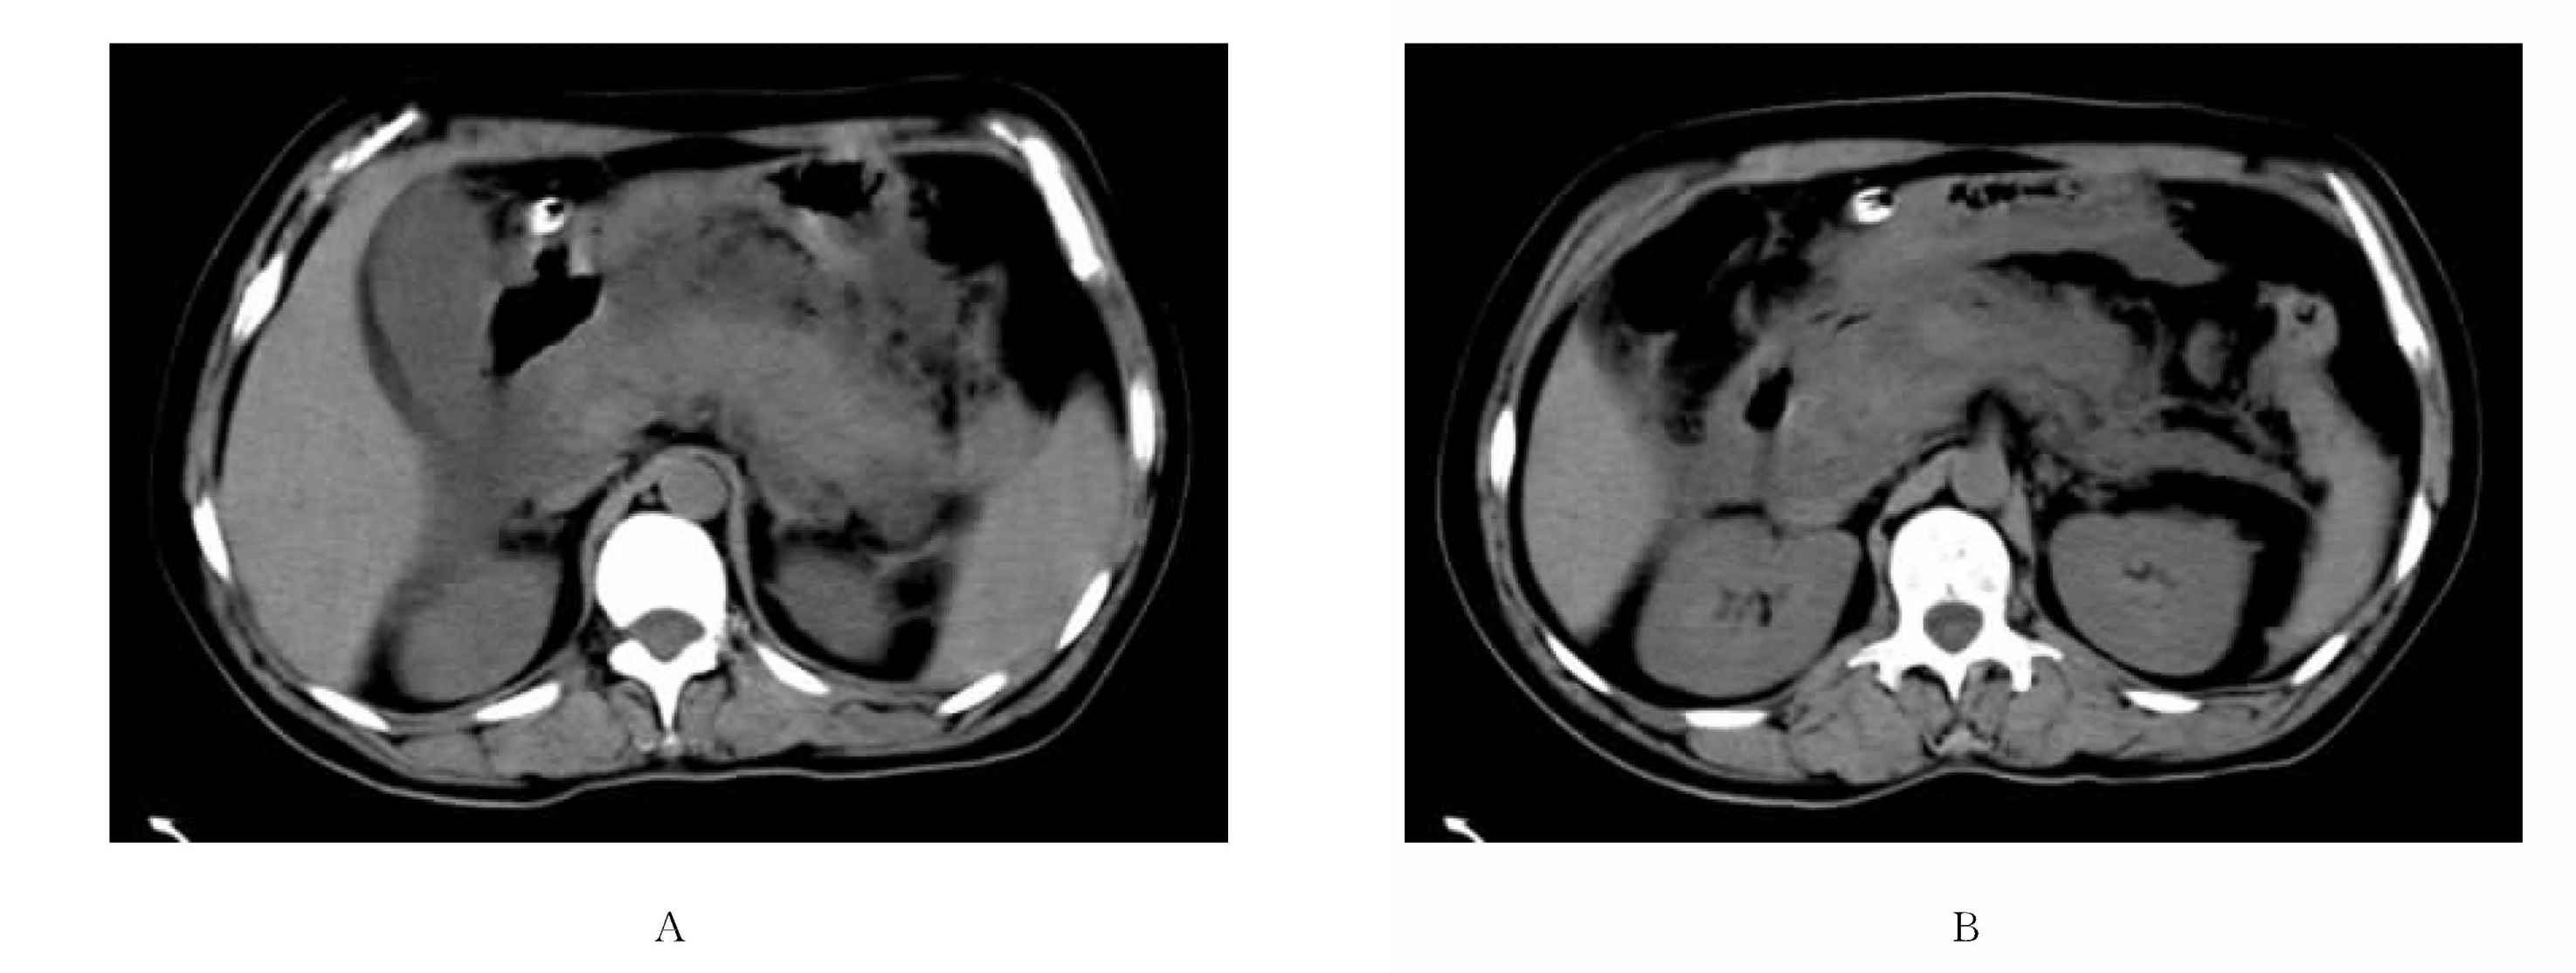
\includegraphics[width=.7\textwidth,height=\textheight,keepaspectratio]{./images/Image00300.jpg}
 \captionsetup{justification=centering}
 \caption{急性胰腺炎\\{\small A、B为同一患者,胰腺体积增大,边缘模糊,周围有大片水样密度区,左肾筋膜增厚}}
 \label{fig13-1}
  \end{figure} 

\textbf{【并发症】} 急性胰腺炎尤其是坏死性胰腺炎的并发症有:

1.胰腺内或胰周积液:胰腺周围缺乏坚固而完整的包膜,胰腺分泌物含有胰酶,很容易突破胰周薄层的结缔组织而进入胰周间隙及肾旁前间隙,形成所谓“蜂窝组织炎”。主要表现为“积液”,实为炎性混合物。积液代表着假性囊肿或脓肿的早期形成,大约40%~50%积液在5~6周自发性吸收,6周后则常发展为假性囊肿或脓肿。

2.假性囊肿:其形成至少需要4周以上,但也有报道10~20d积液边缘即可形成肉芽组织假膜。CT表现为圆形或卵圆形水样密度灶,有薄层包膜或薄壁,或有强化的厚壁。假性囊肿最常位于胰周,但也可见于整个腹腔、纵隔和盆腔。40%假性囊肿或脓肿可自行消除。

3.胰脓肿:是腹腔内毗邻胰腺的脓液积聚,其内几乎无坏死,通常出现在发病4周后,并且可以是局限性坏死伴继发性液化或感染的一种并发症。CT表现为局灶性低密度积液伴含气泡的厚壁,但气泡是非特异性的,最终诊断需结合临床或穿刺抽吸活检。

4.感染性坏死:是胰腺和(或)胰周有感染性坏死组织。CT表现为胰腺坏死区内气泡,或表现为密度不均的胰周软组织内呈散在分布的腹膜后气体积聚即“气肿性胰腺炎”。但如胰或胰周坏死组织内不含气时则CT不能诊断感染,而需活检证实。

5.胰性腹水:为胰管破裂胰液进入腹膜腔所致。CT可显示游离腹水,确诊需做淀粉酶水平的测定。

6.出血:可位于胰内或胰周。

7.假性动脉瘤及血管狭窄、闭塞。

8.瘘管:在静脉和假性囊肿之间形成,CT难以显示。

9.血栓:如门静脉血栓。

10.脾脏并发症:梗塞、脓肿、破裂、包膜下积液等,以梗塞和包膜下积液多见。重症者可短暂性增大,是因脾静脉阻塞或狭窄、非特异性脾炎所致。

11.左膈下脂肪浸润:国内闵鹏秋等认为是急性胰腺炎的一个有价值征象,而且与病变程度成正相关。

12.呼吸系统病变:胸腔和心包积液、肺底炎症,甚至呼吸窘迫综合征,以及少见的胰腺胸膜瘘。

13.多发性关节炎、骨缺血坏死等。

14.还可见胃肠道淤张、狭窄、瘘管,小肠、横结肠系膜肿胀,腹膜后大血管周围、腰肌筋膜、肾旁后间隙、纵隔受累等。

\textbf{【CT分级】}
目前采用Balthazar的分级标准,将本病分为5级(见表\ref{tab13-1})。

\begin{table}[htbp]
\centering
\caption{Balthazar CT分级标准}
\label{tab13-1}
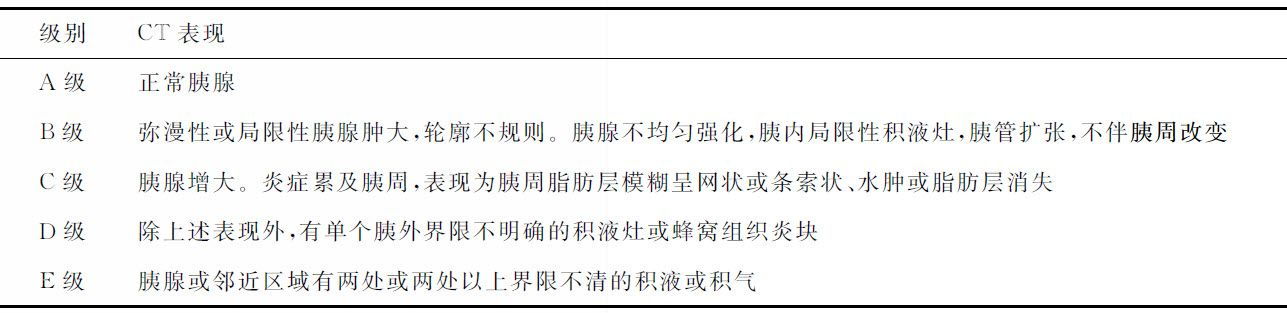
\includegraphics[width=\textwidth,height=\textheight,keepaspectratio]{./images/Image00301.jpg}
\end{table}

\subsection{慢性胰腺炎}

其病因和发病机理比较复杂,意见尚不统一。

\textbf{【病因病理】}
最常见的是胆道疾病及酒精中毒,其他还有急性炎症反复发作、营养不良、高钙血症(甲状旁腺功能亢进)、遗传性因素和结石等。偶尔也可由胆管硬化、胰腺特发性纤维化或肾功能衰竭引起。病理特点为胰腺纤维化,质地变硬、体积缩小、正常小叶结构丧失;晚期腺体完全萎缩,被纤维和脂肪组织取代,胰岛组织也遭受破坏。其改变可为局限性、节段性或弥漫性,伴有胰管不同程度的扩张。

\textbf{【临床表现】}
上腹痛向背部放射,其疼痛可以很严重,也可以完全无痛。视其功能受损的不同其临床表现也不同,常伴有胰腺功能不全的症状如糖尿病、消化不良、脂肪泻、吸收不良和消瘦等。

\textbf{【CT表现】}
①胰腺体积变化:可正常、缩小或增大。增大表明有炎症水肿存在或伴有囊肿,多为弥漫性,少数为局限性。萎缩可为局限性或完全性,伴或不伴脂肪取代。弥漫性萎缩亦可见于糖尿病人,还需注意与老年生理性改变区分。②胰腺及胰管钙化:呈星形、条状或结节状,甚至呈全胰腺钙化,对慢性胰腺炎的诊断有一定特征。但钙化亦可继发于脂肪坏死、出血等,还需与胰腺结核和胰腺结石相鉴别。③胰管扩张:多呈不规则串珠状,或狭窄与扩张交替存在,也可呈管状扩张。少数伴胆总管的炎症性狭窄和近端扩张,表现为胆总管由上至下逐渐变细。④可见胰腺内或胰周囊肿、血管受累等继发改变(图\ref{fig13-2})。⑤可有左肾前筋膜的反应性增生。⑥有2%~5%的慢性胰腺炎合并胰腺癌。

\begin{figure}[!htbp]
 \centering
 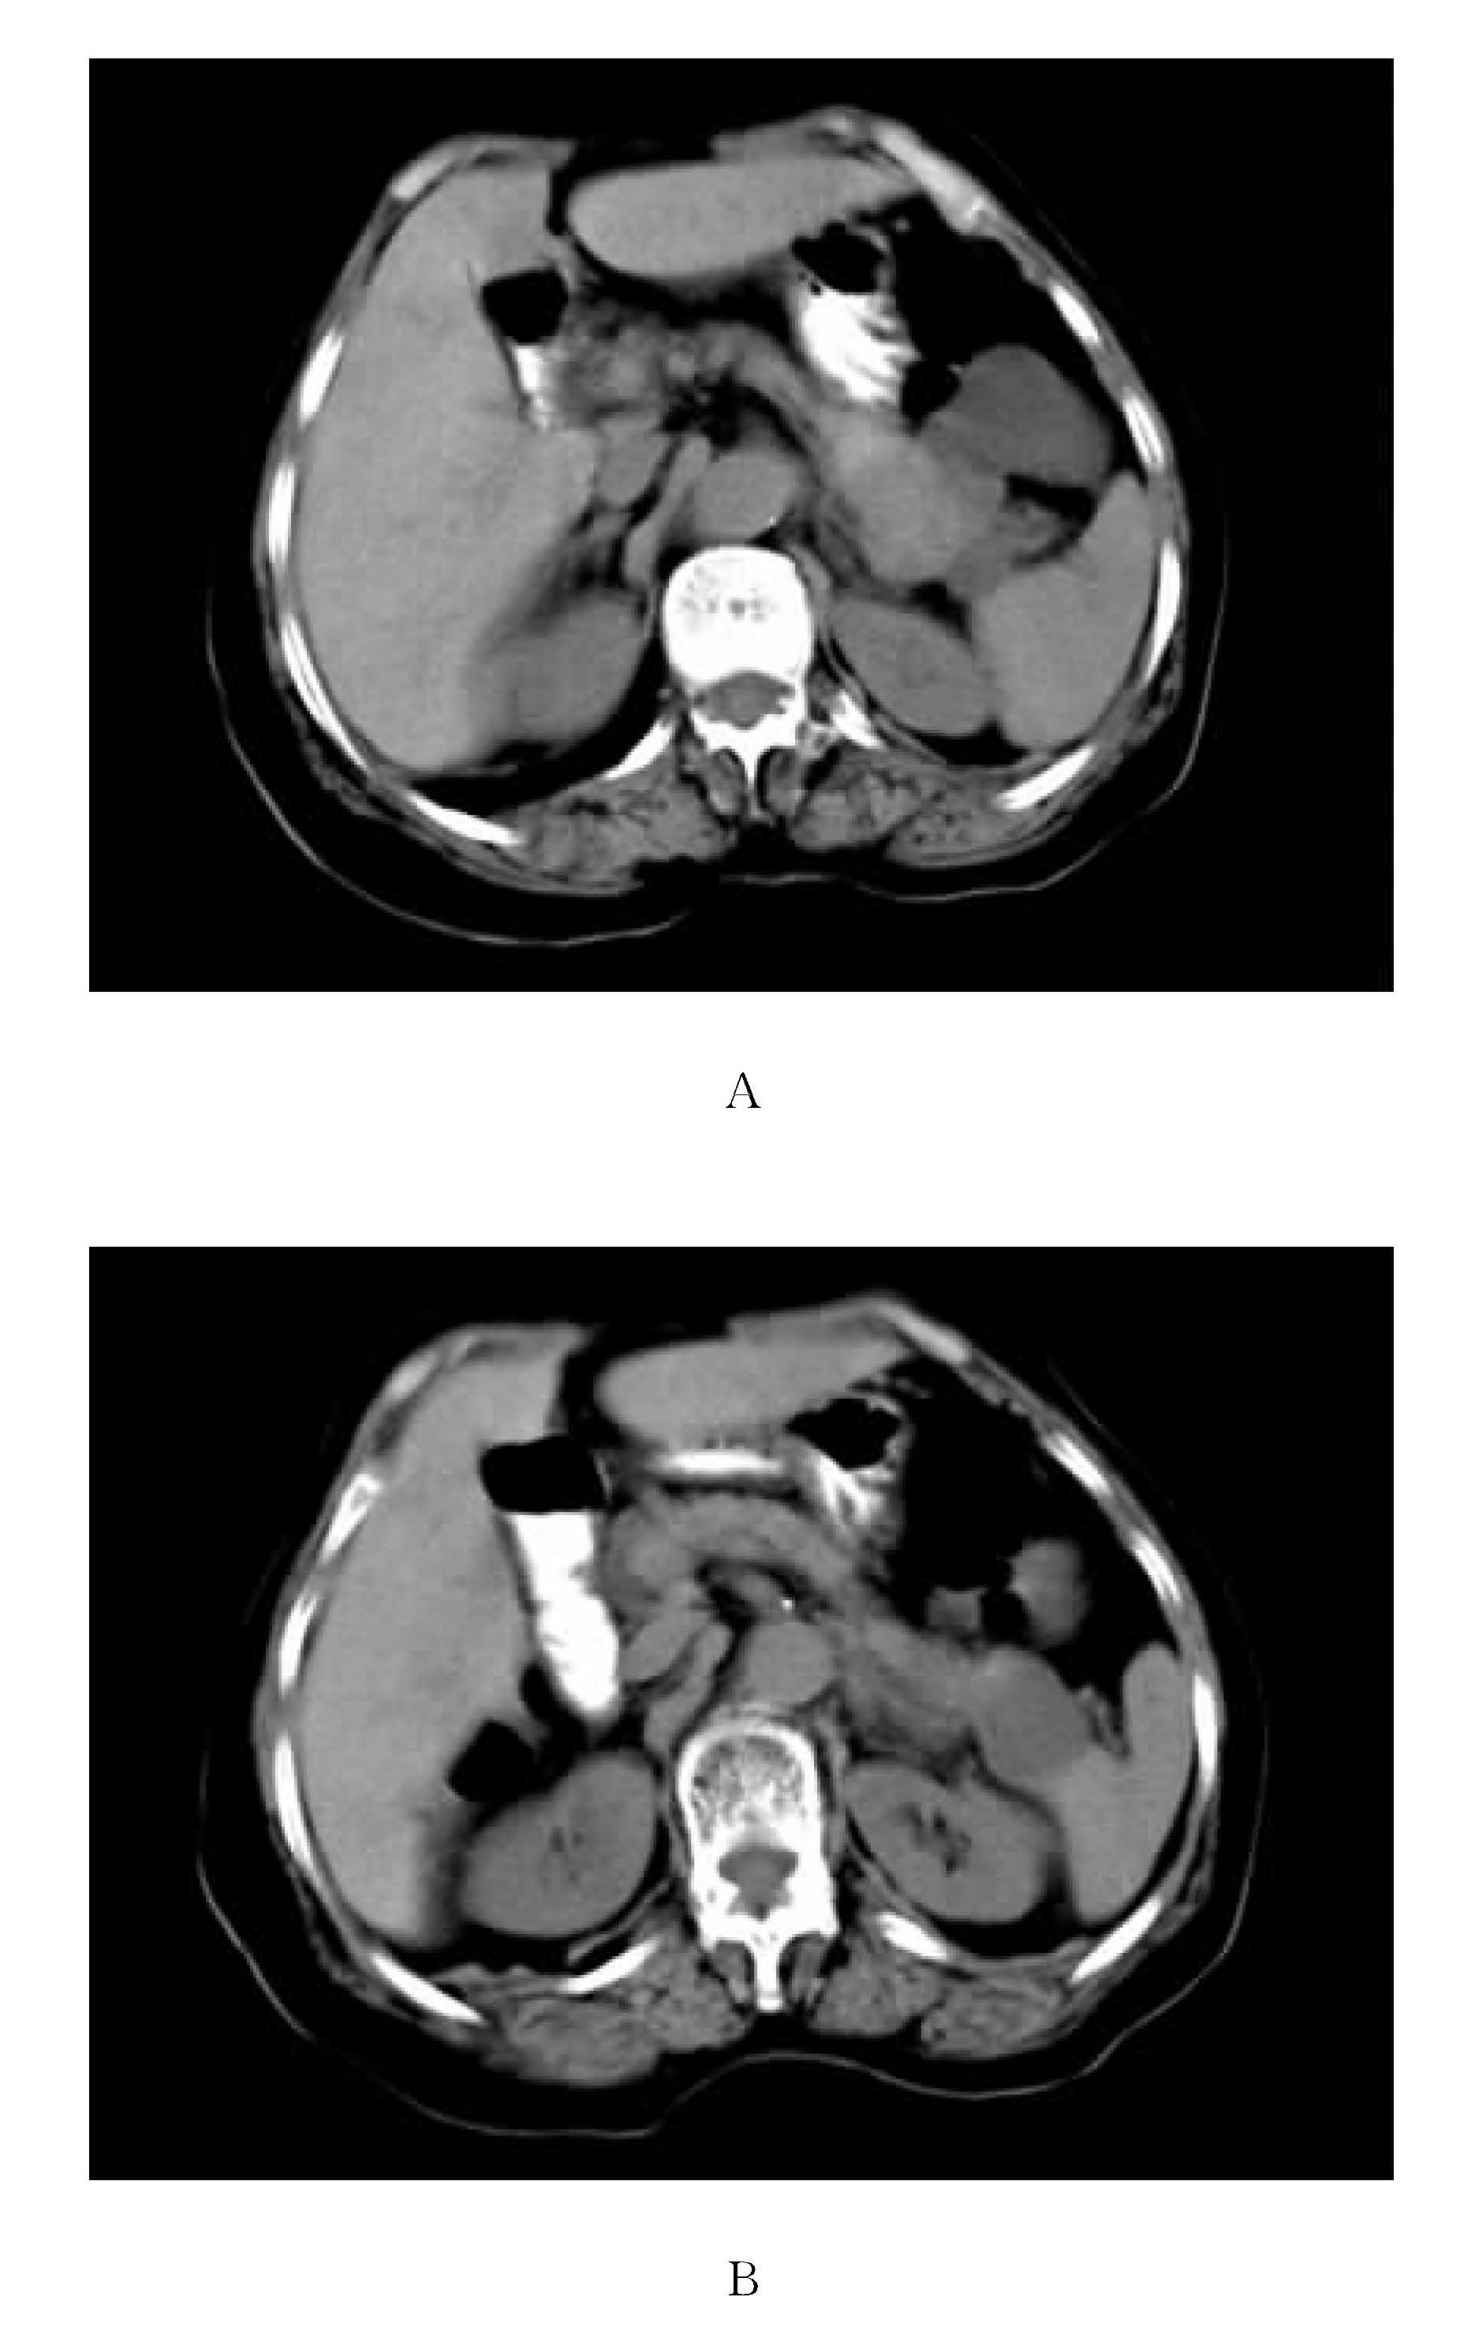
\includegraphics[width=.7\textwidth,height=\textheight,keepaspectratio]{./images/Image00302.jpg}
 \captionsetup{justification=centering}
 \caption{慢性胰腺炎之假性囊肿\\{\small A、B为同一患者,胰尾前方和胰尾部有囊状水样密度灶}}
 \label{fig13-2}
  \end{figure} 

\subsection{假肿瘤性慢性胰腺炎}

本病又称为局灶性胰腺炎,占慢性胰腺炎的10%~36%。其特点是胰腺实质肿块形成,与胰腺癌的鉴别极为困难,有时甚至是不可能的。肿块93%位于胰头部,可能与此处胰管的解剖分布特点有关。

\textbf{【临床表现】}
90%~92%有慢性酒精中毒,至少有6年以上饮酒史;85%有慢性胰腺炎反复发作史。当肿块位于胰头时,54%出现间歇性黄疸。85%可触及肿块,肿块质地较硬。

\textbf{【CT表现】}
①密度:77%~83%较均匀,略高于胰腺实质。②强化特点:多因丰富血供,92%明显强化,其中25%高于邻近胰腺实质,67%类似于邻近胰腺实质,强化后CT值升高20~50Hu,此点有别于乏血的胰腺癌。8%无明显强化,可能由于慢性胰腺炎晚期,动脉内膜下或中层纤维化、增厚、管腔狭窄、肿块血供差有关。③形态:多呈圆形或类圆形,边缘多规则,>5cm时欠规则。④胰腺周围血管间隙内脂肪受浸润:60%可见此征,故此征并非仅见于胰腺癌。⑤肠系膜上动、静脉管径的变化:胰腺炎时肠系膜上静脉扩张,而胰腺癌时肠系膜上动脉直径增大。因此,当肠系膜上动、静脉比值>1时应警惕胰腺癌,反之,则提示良性病变。⑥钙化:47%~67%假肿瘤性肿块有钙化。⑦53%炎性肿块压迫胰管致其不规则串珠状扩张,并可见胰管内结石。局限性慢性胰腺炎20%可见双管征,而90%的胰腺癌有此征,应注意鉴别。

\subsection{胰腺结石}

临床上将胰腺结石分为两大类:①胰管结石:又称真性结石,需手术治疗;②胰实质内钙化:又称假性结石,不需手术治疗。

\textbf{【病理】}
胰管结石多位于胰头部胰管内,呈鹿角形,并嵌顿(术中所见)、阻塞胰管,致胰液引流不畅、胰管扩张,甚至胰管极度扩张使整个胰腺呈囊状;胰管结石加重胰腺的慢性炎症改变,在胰腺慢性炎症的基础上可并发胰腺癌。胰实质内钙化多位于体、尾部。

\textbf{【临床表现】} 一般有慢性胰腺炎病史及其临床表现。

\textbf{【CT表现】}
胰管结石的特征是胰头部大片状高密度钙化并胰管明显扩张,有时可见胰头部增大,边缘模糊。而胰腺实质钙化多位于体、尾部,较前者分散,也可呈片状,一般不伴胰管扩张。

\subsection{自身免疫性胰腺炎}

本病又称为硬化性胰腺炎、胰腺慢性炎性硬化等。其临床特点、治疗及预后与一般慢性胰腺炎均有不同之处。

\textbf{【病因病理】}
本病与免疫异常有关。其病理学特点为胰腺弥漫性肿大及纤维化;胰腺弥漫性淋巴细胞、浆细胞浸润,腺泡萎缩,组织间隙纤维化,并可累及腹膜后胰周组织。

\textbf{【临床表现】}
本病以50岁以上的男性多见。常无明显的临床症状,偶有上腹部或后背部轻度不适,常被忽略。病变发展到后期,因胆总管胰腺段狭窄导致进行性加重的无痛性黄疸。实验室检查有不同程度的肝功能受损,还有高丙种球蛋白血症、血清IgG水平升高、自身抗体阳性,CA19-9水平可升高,但多低于胰腺癌患者。

\textbf{【影像学表现】}
胰腺弥漫性或局限性增大,胰周渗液较少且局限,肾筋膜可增厚。CT显示肿大胰腺边缘平直,MR平扫显示胰腺实质信号不均。增强扫描病变区域胰腺实质呈均一性延迟强化。如炎症较局限则表现为局部软组织肿块,很难与肿瘤相鉴别。本病常累及胆管,表现为胆管节段性狭窄,其近端肝内外胆管扩张,呈残根状表现;胰管不规则狭窄。

本病与常见的慢性胰腺炎胰腺体积缩小、腺实质钙化、假囊肿形成、胰管串珠状扩张等明显不同。但由于本病的临床症状和检查缺乏特征性的表现,影像学又甚似肿瘤或普通慢性胰腺炎,所以诊断十分困难。

综合国内外文献,大多数患者具有如下特征:①血清γ球蛋白水平升高或IgG水平升高,特别是IgG4;②自身抗体阳性;③胰腺弥漫性肿大;④弥漫性胰腺主导管不规则狭窄伴胆总管下段狭窄;⑤伴淋巴细胞、浆细胞浸润的纤维化;⑥无症状或症状轻微(与急性胰腺炎有别),伴无痛性黄疸;⑦罕见胰腺钙化或囊肿;⑧偶伴有其他自身免疫性疾病;⑨激素治疗有效。

\subsection{胰腺结核}

本病少见,一般由淋巴、血行传播而感染。

\textbf{【临床表现】}
常有结核中毒症状。腹痛、腹部压痛是最常见的症状和体征,发生率超过半数,尤其腹部压痛常提示炎性病变。也可有阻塞性黄疸、腹泻、体重下降等。实验室检查最常见血沉增快、OT试验或PPD试验绝大多数呈阳性反应。

\textbf{【CT表现】}
本病好发于胰头,体尾部亦可发生,亦可累及整个胰腺。可为局灶型、多结节型及弥漫型,以局灶型最常见,并以胰腺局灶性蜂窝状强化为特征。

1.胰腺局灶性肿块:多位于头颈部,直径从数cm至10cm不等。病灶呈低密度(干酪或增殖性病灶),当部分液化时呈囊实性肿块,完全液化时呈囊性病变,常有多数分隔。病程长者可有钙化。增强扫描周边及分隔可有不同程度的强化,且无壁结节是其特征。

2.胰腺内多发结节:表现为整个胰腺不规则结节样增大,其内可见多个灶性低密度区。增强扫描见结节状病灶周边强化,结节本身无强化或轻度强化。此型可能为血行播散感染表现。

3.胰腺弥漫性增大:胰腺密度普遍降低,边缘模糊,与胰腺炎类似。增强扫描呈不均匀强化。可能为粟粒型胰腺结核病灶小而难以显示,或反应性胰腺炎。常伴胰周淋巴结增大、融合,并呈花环状强化。

4.胰外表现:①淋巴结增大:最常见。平扫呈低密度结节,增强扫描呈环状或花环状强化,部分有斑片状或环状强化。②腹腔实质脏器受累:可伴肝、脾增大,包括反应性增大和结核浸润,前者更多见。③尽管肺结核多见,但胰腺结核伴活动性肺结核者并不多见。偶见胸水、肺浸润灶、纵隔淋巴结增大。④常有腹水表现。

总之,胰腺内局灶性蜂窝状强化的肿块、胰周及门静脉周围淋巴结增大伴周边环状强化,以及其他结核播散灶是本病的主要CT表现。应注意与胰腺癌、囊腺癌、恶性淋巴瘤、转移性肿瘤和脓肿等鉴别。

\section{胰腺肿瘤}

\subsection{概述}

胰腺肿瘤按组织学分为两大类。①胰导管细胞肿瘤:最常见的是导管细胞癌,占82%以上;其他为浆液性囊腺瘤、黏液性囊腺瘤或癌、导管内乳头状瘤和胰腺类癌。②非导管细胞肿瘤:极少见,包括内分泌肿瘤、胰母细胞瘤、平滑肌肉瘤、神经母细胞瘤、纤维瘤、纤维肉瘤、血管球瘤、脂肪瘤或脂肪肉瘤、淋巴瘤和囊性畸胎瘤等,胰腺转移瘤也较罕见。

胰腺恶性肿瘤又可分为两大类:①原发性:其组织学分类尚未统一(见表\ref{tab13-2})。②转移性:包括血源性、直接侵犯和淋巴源性。

\begin{table}[htbp]
\centering
\caption{胰腺原发性恶性肿瘤的分类(Cubilla分类法)}
\label{tab13-2}
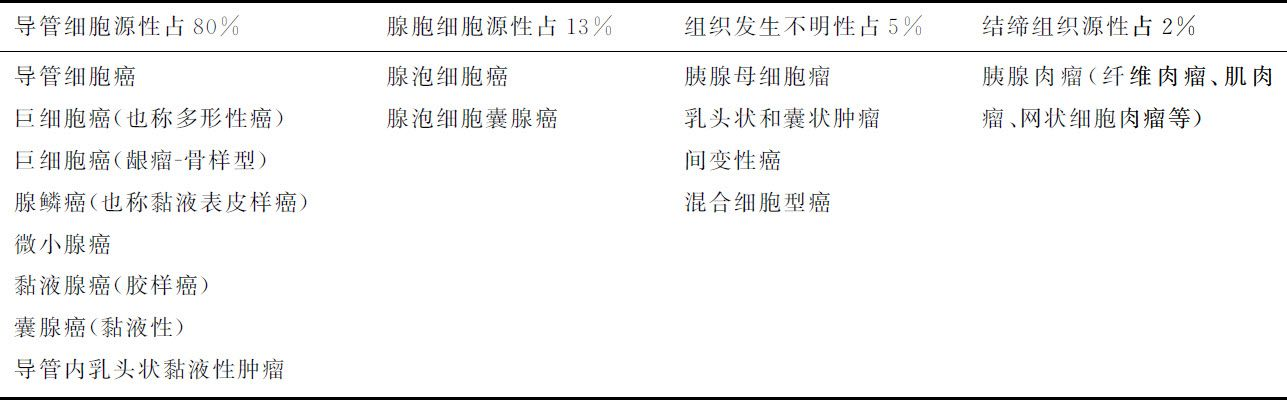
\includegraphics[width=\textwidth,height=\textheight,keepaspectratio]{./images/Image00303.jpg}
\end{table}

\subsection{胰腺癌}

本病近年来有明显上升趋势。

\textbf{【病理】}
主要为导管细胞源性的导管细胞癌(好发于胰头),其次为腺泡细胞癌(好发于胰体尾),两者均属于腺癌。其他为少见的囊腺癌等。胰腺癌胰头部占60%~70%,体部约10%~15%,胰尾部约占5%;有时弥漫性分布于胰腺各部属弥漫性胰腺癌,约占15%~20%。病灶呈坚硬的结节样肿块,与周围胰腺界限不清,较大时易变性坏死。因胰腺癌通常发生于胰管上皮,且具有围管式生长和嗜神经性生长(向后方)的特性,因此常伴胰管及胆管阻塞,造成梗阻远端胰管局限扩张和胰腺萎缩,有时可在胰内形成潴留性囊肿。胰腺癌常侵及邻近血管结构,甚至侵及胃、十二指肠等脏器。

转移途径:由于胰腺癌生长较快,胰腺又无包膜,往往早期发生转移。①血行转移:以肝脏最常见,其次为肺、肾上腺、肾等。②淋巴转移:胰十二指肠后、胰头上下、胰体上、胰十二指肠前等近胰淋巴结群,以及胃幽门下、肠系膜上血管根部、腹膜后大血管周围等远胰淋巴结群,偶可见锁骨上淋巴结转移。③腹膜种植:可达20%~30%。

\textbf{【临床表现】}
多见于中老年人,男女之比约1.8∶1,偶见于儿童。①腹痛:约半数以腹痛和腹部不适为最早出现的症状。②黄疸:无痛性黄疸为其最突出的症状,黄疸呈持续性、进行性加重,也可有波动。少部分早期甚至中、晚期亦无黄疸。③其他:消瘦、纳差、乏力和恶心呕吐等,脏器转移者可出现相应临床症状。

\textbf{【CT表现】}

\subsubsection{直接征象}

1.胰腺内低密度或等密度肿块:伴或不伴胰腺轮廓改变(图\ref{fig13-3}A)。90%境界不清,52%呈等密度,约6%远段萎缩,3%有钙化。

2.增强扫描:本病为少血管性肿瘤,故肿块强化不明显呈低密度;若肿块内部已发生坏死液化时,则呈更低密度。而正常胰腺实质可明显强化且密度均匀。对胰腺癌的检出以实质期(40s)增强扫描为佳(图\ref{fig13-3}B~D)。

\begin{figure}[!htbp]
 \centering
 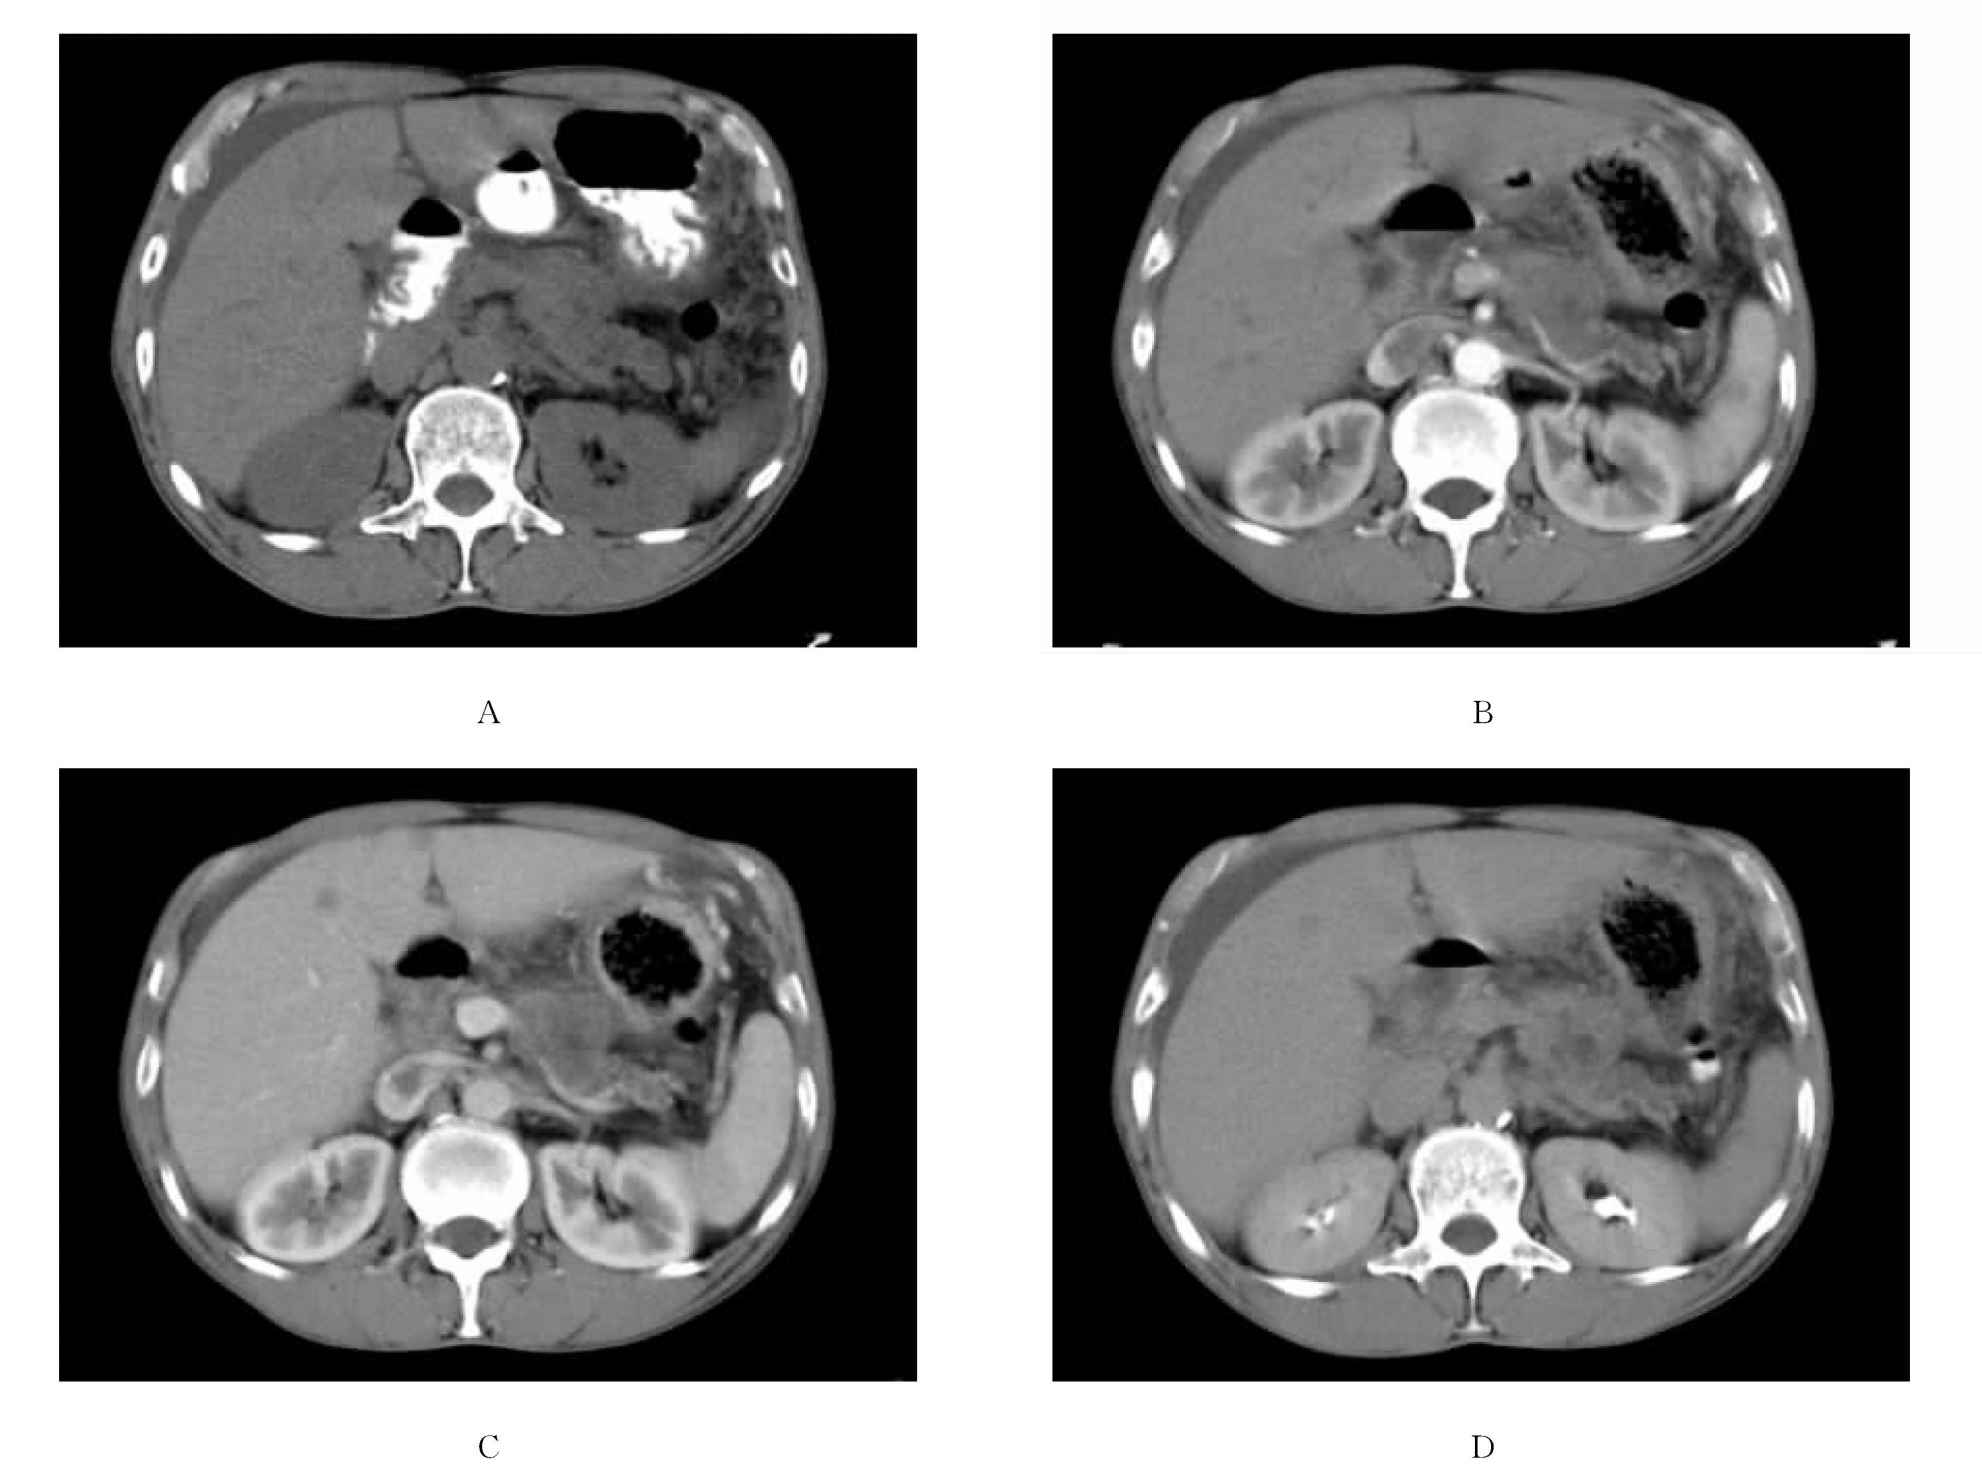
\includegraphics[width=.7\textwidth,height=\textheight,keepaspectratio]{./images/Image00304.jpg}
 \captionsetup{justification=centering}
 \caption{胰腺癌(体部)\\{\small A~D为同一患者。A为平扫,B为动脉期,C为门静脉期,D为平衡期;平扫胰体部不规则增大;增强扫描胰体部肿块无明显强化,其内有更低密度坏死区;肝周有腹水}}
 \label{fig13-3}
  \end{figure} 

国内有学者认为,对瘤体供血起绝对主导作用的是瘤体内残存胰腺组织的微血管,高分化胰腺癌残存胰腺组织多,以等密度强化为主;中、低分化者残存胰腺组织相对减少,呈低密度强化,而且低分化者易伴有囊状、不规则大片状低密度坏死区。

3.较大的肿瘤可造成胰腺轮廓或外形的改变,表现为局限性膨大、突出的肿块影,边缘呈分叶状;较小的肿瘤(直径≤2cm),特别是瘤体位于中心区域时,可不造成轮廓或外形的改变,故增强扫描对显示肿瘤尤为重要。

4.在观察胰腺增大、轮廓及外形改变时应注意:①不应单纯依赖测量径值,应注意观察胰腺由头至尾各部比例是否协调,结合增强扫描是否有低密度灶尤为重要。②胰头部肿瘤常常仅出现局部圆隆或球形扩大,而不像胰体尾部的肿瘤局部显著扩大和分叶状,但若伴有体尾部继发性萎缩,则这种球形扩大易于显示。③钩突正常为楔形,钩突肿瘤可使其圆隆或呈分叶状增大,突出于肠系膜上血管与右肾静脉之间,甚至包绕肠系膜上血管。④全胰浸润性胰腺癌者,表现为胰腺弥漫性不规则增大,有时伴不规则低密度或混合密度。⑤老年人胰腺趋向萎缩且密度低,如外形不小,轮廓僵直、锯齿缘轮廓消失,密度又高,则应疑诊胰腺癌可能。

\subsubsection{间接征象}

其间接CT征象包括胰周组织结构的受侵和远处脏器的转移灶等,在前者以向腹膜后的局部扩展尤为常见。

1.胰腺周围血管受累:主要包括腹主动脉系的腹腔动脉干、肠系膜上动脉及脾动脉,门静脉系的门静脉起始部、脾静脉和肠系膜上静脉,以及下腔静脉等。其表现为:①胰周血管的脂肪层消失;②胰周血管被肿块包绕(范围超过180°)或包埋于肿块内;③胰周血管形态异常如变细、边缘不整齐等,以及走行异常如僵直、被推挤等;④受累血管不显影或管腔扩大,有时可见腔内软组织密度的癌栓;⑤可发现代偿性的静脉侧支循环建立。

2.胰腺周围脏器受累:主要表现为与有关脏器的正常脂肪层模糊、消失。①对空腔脏器而言,如同时出现相应管壁的不规则、结节样增厚,则高度提示受累。②肝、脾门结构紊乱,相邻实质内出现低密度灶,也提示有肿瘤侵蚀。

3.梗阻性胆管扩张:呈突然性不规则狭窄、管腔截断消失、管腔内软组织结节并与管外胰内病灶相连等,部分可无肝内外胆管扩张。

4.胰管扩张:发生率约50%~60%(还有报道高达80%)。①扩张的胰管多呈平滑状,偶可呈串珠状,在胰头内呈圆形管状断面。多在胰头肿块处截断。②如与扩张的胆总管(位于扩张胰管的后外侧)并存则形成“双管征”(图\ref{fig13-4})。③胰体尾的胰管扩张常伴体尾部萎缩。④胰管某段的局限性扩张,应警惕早期胰腺癌。

\begin{figure}[!htbp]
 \centering
 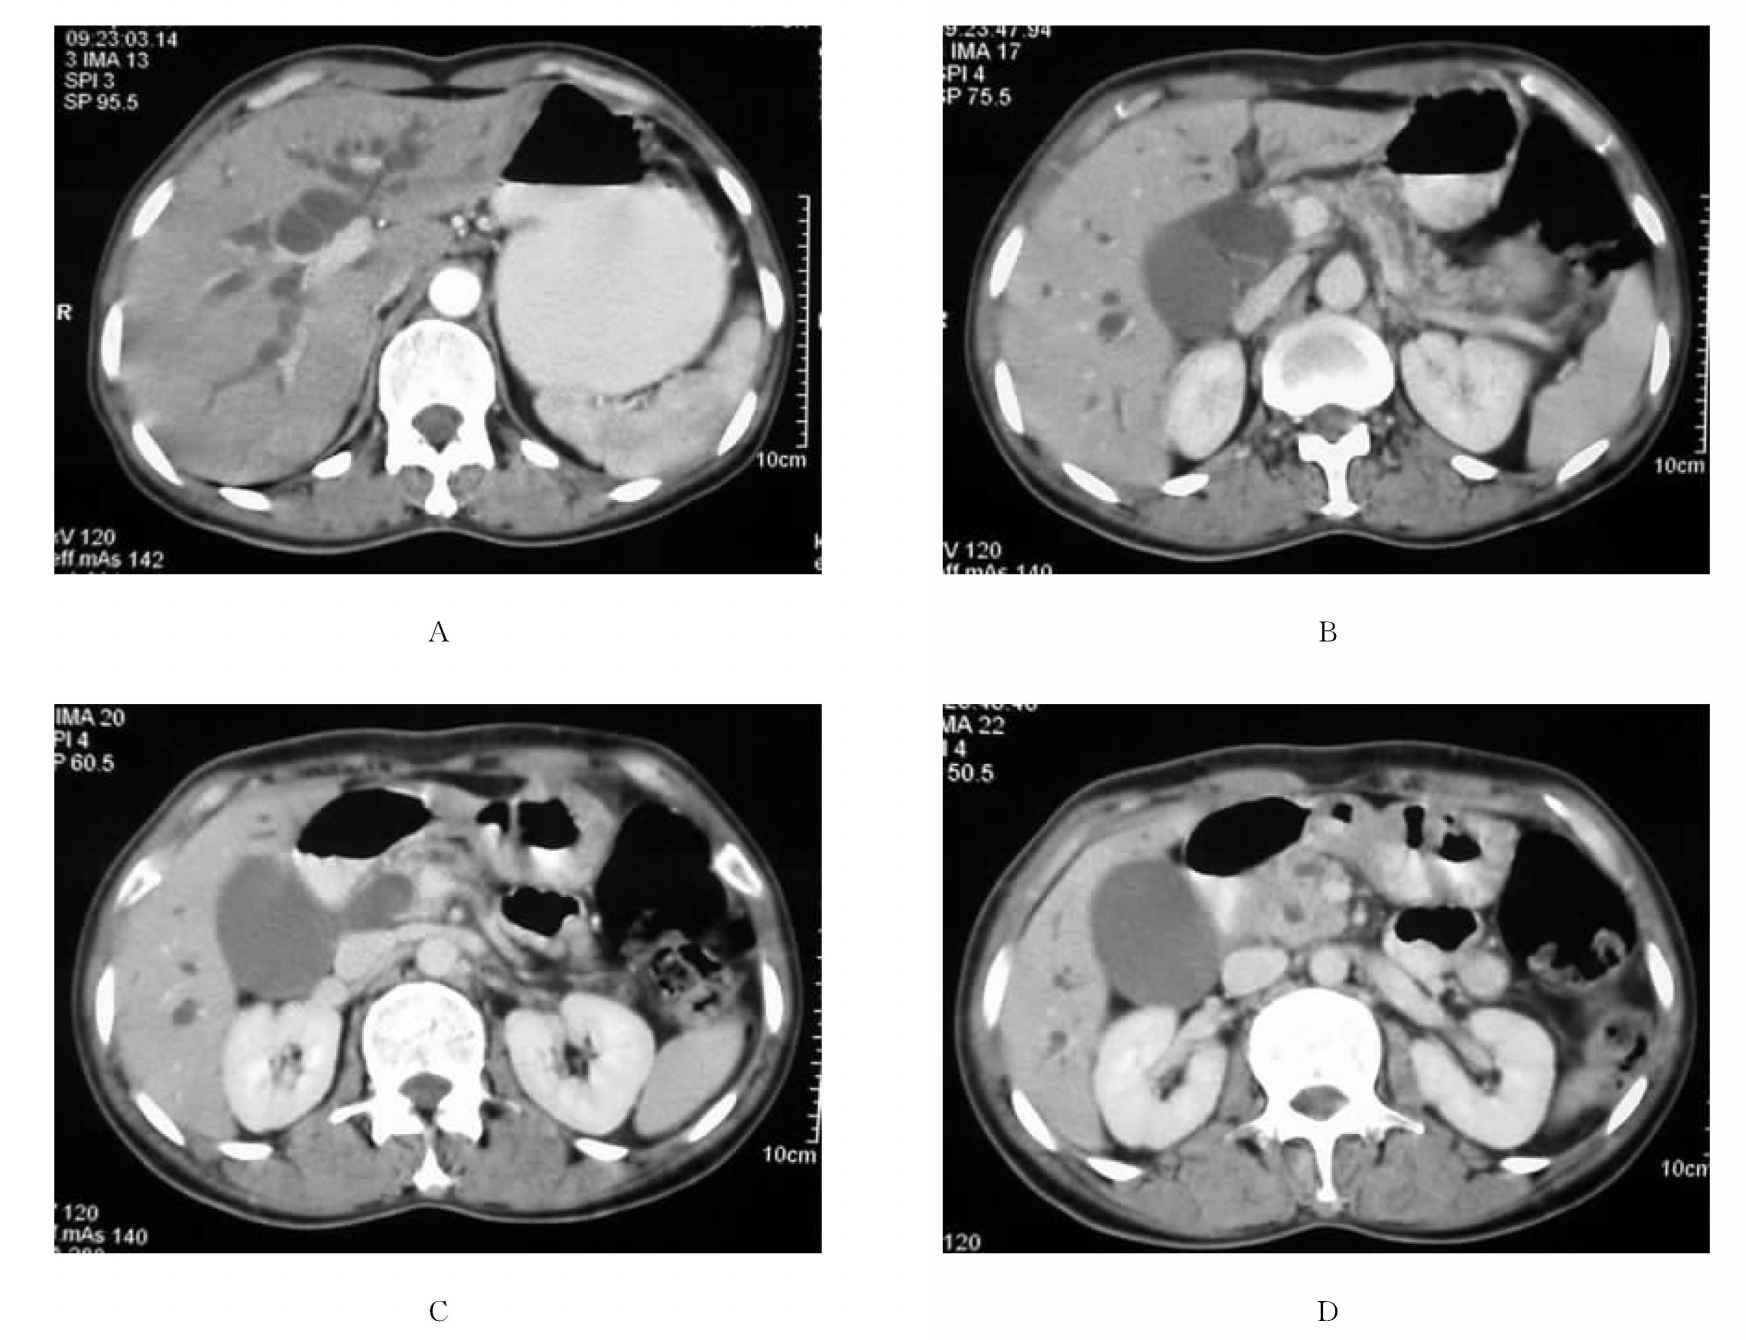
\includegraphics[width=.7\textwidth,height=\textheight,keepaspectratio]{./images/Image00305.jpg}
 \captionsetup{justification=centering}
 \caption{胰头癌\\{\small A~D为同一患者,增强扫描表现。可见肝内外胆管扩张、胰管扩张(双管征),钩突增大}}
 \label{fig13-4}
  \end{figure} 

5.继发性潴留囊肿:呈圆形或球形水样低密度,常位于肿瘤远侧胰腺组织内,少数位于胰周。

6.胰周淋巴结转移:可单个或融合成块,密度均匀,中心坏死出现较晚,亦可侵犯邻近血管。

7.脏器血行转移:肝转移发生率50%以上,其他有肺、肾上腺、肾等。

8.腹膜种植:一般较小,呈粟粒结节状,CT难以显示。偶见腹膜不均匀增厚,以及网膜、系膜软组织结节,甚至“饼状”网膜等征象。腹水一般出现较晚。

\subsubsection{早期胰腺癌的诊断标准}

有关早期胰腺癌的定义尚存在争议,多认为其诊断标准为:①肿块最大径≤2.0cm;②胰周脂肪及被膜无受累;③胰周血管无受累;④无胰周区域淋巴结、远处淋巴结转移,也无肝及其他邻近或远处脏器转移。还有学者认为应将肿瘤最大径≤1.0cm作为划分标准,原位癌或有微小浸润的管内癌,不论其大小,也列入早期胰腺癌的范畴。

早期胰腺癌除了显示低密度肿块的直接征象外,其间接征象的显示如胰管、胆管的扩张,胰腺体尾部萎缩,胰腺形态或轮廓的改变亦很重要。诚然,亦可无肝内外胆管的扩张,或仅显示轻微的胰管扩张。还有作者报道几例无或仅有轻微浸润的早期胰腺癌的惟一CT征象是主胰管或分支胰管的扩张。

\textbf{【鉴别诊断】}

1.慢性局限性胰腺炎:典型的临床表现、病史过程和典型CT表现大多可以鉴别慢性胰腺炎和胰腺癌,但与不典型者尤其胰头或钩突增大的局限性(或称肿块型、假肿瘤型)慢性胰腺炎鉴别常十分困难。

下列表现提示慢性胰腺炎可能大:①胰头、钩突区出现钙化,胰管内或胆总管内结石;②胰头、钩突增大,但外形规整、光滑,一般无分叶征;③强化后胰头、钩突区密度均匀或稍欠均匀,不易出现像胰腺癌那样的低密度结节或肿块(合并小假性囊肿者除外);④胰周血管、邻近脏器无恶性侵犯表现;⑤胰头部胆管虽可扩张,但逐渐变细,无突然截断、变形表现。

但上述征象除①外均不可靠,且胰腺癌可发生于慢性胰腺炎基础上,又进一步增加了鉴别诊断的难度。

2.胰腺囊腺瘤(或癌):较少见,组织学上囊腺瘤属良性,而囊腺癌属恶性。CT表现为:①大小不等、单发或多发的、边界清楚或不清楚的囊实性肿块。②囊内密度一般均匀,存在分隔,囊壁可见壁结节。部分还可见囊中央放射状纤维瘢痕征象,是浆液性囊腺瘤的特征。③有时囊壁或囊内容物可出现钙化。④增强扫描可见囊壁及纤维分隔有中度强化,与乏血的胰腺癌有别。

3.胰岛细胞瘤:多为良性,少数为恶性。其最显著的病理特点在于富血供。增强扫描病灶显著强化,尤以动脉期显示为佳。结合临床、实验室检查不难诊断,并可与胰腺癌鉴别。

4.转移性肿瘤:消化道肿瘤、乳腺癌、肺癌等均可发生胰腺实质内转移或胰周淋巴结转移。CT表现为胰腺实质内或胰周多数融合成团的低密度灶,与原发性胰腺癌难以鉴别。需结合病史及临床综合诊断。

\subsection{胰腺囊腺瘤或囊腺癌}

胰腺囊腺瘤(或癌)并不多见,约占所有胰腺肿瘤的10%~15%;恶性者占恶性肿瘤的5%,是胰腺癌的一种特殊类型,且与胰腺癌有不同的病理和CT表现。目前将其分为两大类,但以黏液性囊性肿瘤多见。

\textbf{【病理】}

1.浆液性囊腺瘤:也称微小囊腺瘤或富糖原囊腺瘤,无恶变倾向,胰腺亦无原发性浆液性囊腺癌这一疾病。可发生于胰腺各个部位。肿块单发多见,由多数微小囊肿组成,小囊直径从数毫米至2cm不等,一般<2cm。小囊数目从数个至无数,典型者切面呈“蜂窝状”改变。囊液为浆液性,富含糖原。有时肿块中心存在纤维瘢痕灶,呈辐射状,中央瘢痕可发生钙化。

2.黏液性囊性肿瘤:又称为巨囊性肿瘤。可分为黏液性囊腺癌(具有明显恶变表现)和黏液性囊腺瘤(有潜在恶变性,可恶变为囊腺癌)。黏液性囊性肿瘤起源于胰管上皮,多位于胰体、尾部,偶位于钩突。常为单发,肿瘤一般长得较大,瘤体有完整包膜,外表光滑,分叶清楚。切面呈单囊或多囊性、单房或多房性。囊肿一般>2.5cm,数目一般不超过10个。囊壁厚薄不均,局部可见富血供的壁结节,囊壁或包膜可出现钙化。囊内含大量混浊黏稠黏液,囊之间可有较纤细间隔。黏液囊腺癌的恶性细胞常局限于整个瘤体的某一部分,故穿刺活检可漏诊。肿瘤直径>5cm要考虑恶性可能,>8cm多为恶性。

\textbf{【临床表现】}
两类均好发于中老年女性。上腹部不适、隐痛及腹部包块为主要表现,偶可出现黄疸等消化道症状,或无症状而偶然发现。

\textbf{【CT表现】}

1.浆液性囊腺瘤:①小囊型:呈边界清楚的分叶状囊实性肿物,由多个<2cm的囊构成,囊液呈低密度。小囊之间可见肿瘤的实性部分和纤维间隔,有时可见中央呈星状的瘢痕。②大囊型:呈边界清楚的>2cm的圆形或类圆形病变,通常为单发,中心可见稀少的间隔。③混合型:中心为多发小囊,周边被>2cm的大囊包绕。

增强扫描肿瘤的实性部分和纤维间隔可强化。较特征的表现是囊中央低密度无强化的瘢痕组织和呈辐射状向外延伸的可强化的纤维间隔;瘤体中央瘢痕组织的钙化发生率为30%~46%,特别是放射状钙化亦较有特征(图\ref{fig13-5})。

\begin{figure}[!htbp]
 \centering
 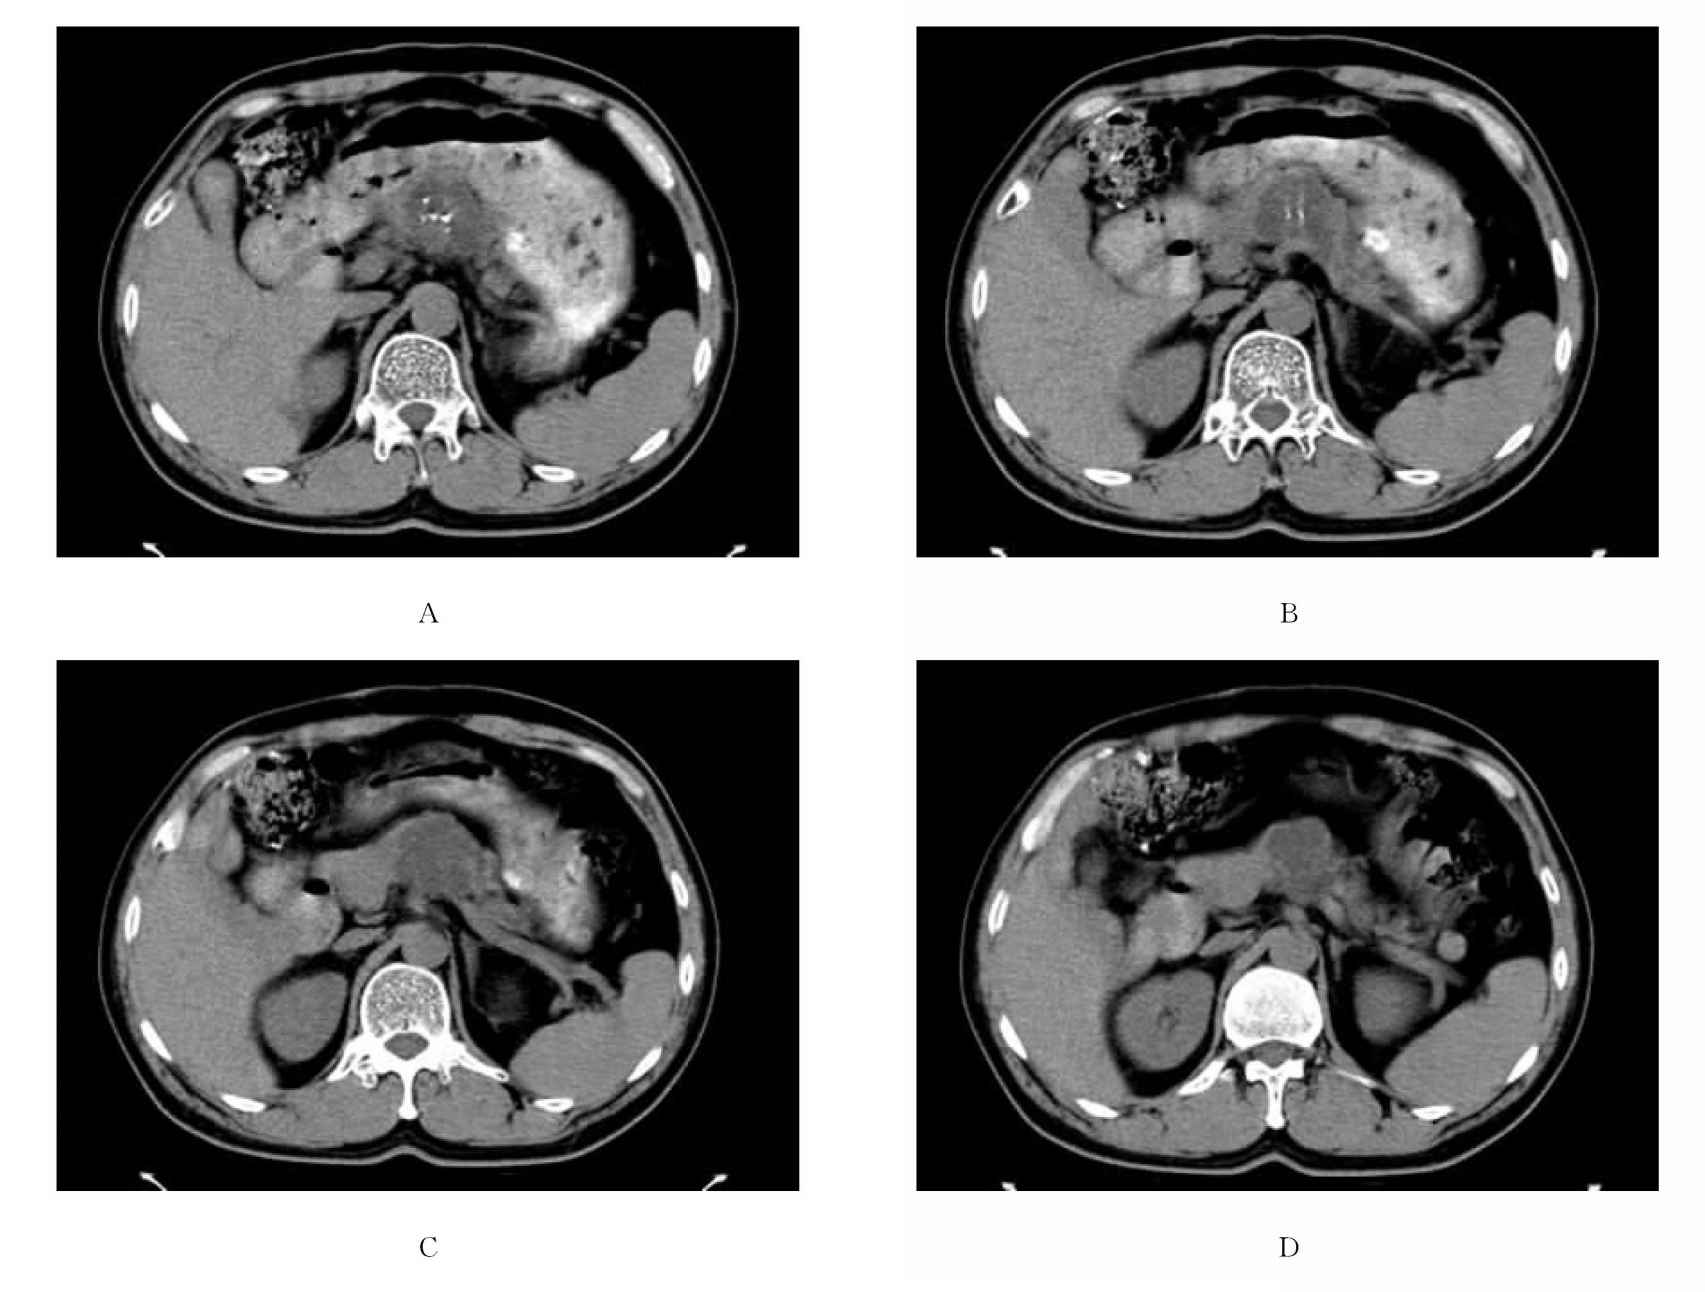
\includegraphics[width=.7\textwidth,height=\textheight,keepaspectratio]{./images/Image00306.jpg}
 \captionsetup{justification=centering}
 \caption{胰腺浆液性囊腺瘤\\{\small A~D为同一患者,胰体部有薄壁囊状低密度灶,界限清晰,其内有沙粒状钙化}}
 \label{fig13-5}
  \end{figure} 

小囊型是其主要类型,大囊型和混合型常需穿刺活检确诊并与其他囊性病变相鉴别。

2.黏液性囊腺瘤(或癌):常为单发囊性肿块,病灶较大,界限清楚,为单房或多房。囊壁厚薄不均匀,可表现为不规则结节状或乳头状的腔内突起,囊内分隔菲薄呈线状或小梁状。囊壁或囊内可出现壳状或不规则钙化,多为外周性分布。国内有报道完全环形钙化、偏侧性条状钙化多为假性囊肿、囊腺瘤,而断续环形钙化,模糊的斑点、条状钙化多为囊腺癌。囊内容物以黏液为主并可含坏死组织,CT值一般较高,约20~45Hu;增强扫描囊壁和壁结节可呈中度以上强化。

此外,黏液性囊性肿瘤如实性成分较多、有明显强化的壁结节、囊壁厚薄不均或厚度>1cm,以及大囊附近多个子囊,则提示黏液性囊腺癌的诊断;若同时出现胰周浸润、淋巴结增大和肝内转移灶等,则更有助于良恶性的鉴别。

\textbf{【鉴别诊断】} 胰腺黏液性囊腺瘤(或癌)应与下列疾病相鉴别:

1.胰腺囊肿:包括先天性囊肿、潴留囊肿和假性囊肿。①假性囊肿:多位于胰外,少数位于胰内。囊壁较薄而均匀,一般无强化,也无壁结节。囊内容物密度均匀,但如有出血、感染或囊壁增厚时二者鉴别困难。②潴留性囊肿:病因常为胰腺癌,如近端发现较确切的实性肿块即可确诊。③先天性囊肿:较少见,壁菲薄,无强化表现,常常是多囊性肾、肝病或(和)脑视网膜血管瘤病的胰腺受累表现。

2.胰腺癌:当出现较大的中央液化、坏死灶时,与黏液性囊腺癌鉴别较困难。但若发现瘤体实性成分较多,壁更厚而不均,囊变区内无分隔现象,以及囊变区内密度混杂不均等征象时,以胰腺癌的可能性大。

3.胰腺囊性淋巴管瘤:有关文献认为,单靠CT表现两者几乎无法鉴别,但囊性淋巴管瘤囊壁菲薄、均匀且无强化,囊内容物多呈水样密度有助于鉴别。

4.胰腺包虫病:典型表现为多囊和囊内分隔,囊内存在子囊,囊周结构强化明显,囊壁可有钙化。结合牧区生活史以及可能合并的肝、肺包虫囊肿等有助于鉴别。

5.胰腺结核:CT表现无特异性,囊壁亦可钙化。胰腺内局限性蜂窝状强化的肿块,以及胰周淋巴结增大、且呈环状强化并融合成簇状或梅花瓣样则支持胰腺结核,结合其他部位播散灶更有助于确诊。

\subsection{胰腺导管内乳头状黏液性肿瘤}

本病是一种少见的胰腺肿瘤,有人认为是黏液囊腺瘤的亚型。1982年Ohhashi最先报道,以往曾被称为胰腺黏液性肿瘤、黏液性导管扩张症、导管内黏液分泌增多性肿瘤、导管扩张性黏液性囊性肿瘤等,1997年WHO正式定名为导管内乳头状黏液性肿瘤。

\textbf{【病理】}
病理及影像学可分为主胰管型、分支胰管型和混合型。本病起源于主胰管或较大分支胰管,呈乳头状生长,表面被覆分泌黏液的柱状上皮细胞,进而胰管进行性扩张,十二指肠乳头增大,黏液可从乳头流入肠腔内。镜下表现为腺瘤、不典型增生或腺癌,三者可相互移行或合并存在,故本病可视为恶性或潜在恶性肿瘤。但发展速度相对较慢,胰周受侵及淋巴结和远处转移均少见,故预后较好。

\textbf{【临床表现】}
发病于30~94岁,平均65.5岁,以60~70岁最多见,男女之比为2.2∶1。其症状有上腹痛、乏力、体重减轻、发热等,亦可偶然发现。大多有慢性胰腺炎病史,亦可以急性胰腺炎就诊,晚期可出现糖尿病。胆总管受累可出现黄疸。实验室检查25.2%CEA增高,45.9%CA-199增高。

\textbf{【CT表现】}
①主胰管型:主胰管弥漫性或节段性扩张,胰腺实质萎缩,胰管内黏液造成密度不均匀增高,其内的乳头状肿瘤可有强化。②分支胰管型:以钩突部多见,病变呈分叶状或葡萄状,由多个直径1~2cm的小囊聚合而成;少数可融合成单一较大囊腔,其中伴有条索状间隔。

但CT对<3mm的扁平状突起难以显示。可有胰管内钙化,但很少见,是由于黏液长期潴留钙盐沉着所致。

\textbf{【鉴别诊断】}
①慢性胰腺炎:主胰管扩张一般伴局限性狭窄,典型者呈串珠状扩张,胰实质内可见粗大钙化或胰管内结石。②胰腺导管癌:围管式生长可导致主胰管远端规则性扩张或胰实质萎缩。增强扫描动脉期或实质期可见低密度的肿瘤区域,胰周有受侵。③经典的胰腺黏液性囊腺瘤:来源于胰腺末梢分支,常突出于胰腺表面,虽可见壁结节和分隔,但周围有纤维包膜,内部以大囊性成分为主,主胰管一般不扩张。本病以中年女性多见,好发于胰体尾部;而导管内乳头状黏液性肿瘤多见于老年男性,好发于钩突部,亦有助于鉴别。

\subsection{胰腺内分泌性肿瘤(胰岛细胞瘤)}

本病亦称胰腺神经内分泌肿瘤。少见,常因产生症状而获得诊断。

\textbf{【概述】}
胰腺中的内分泌细胞称为胰岛细胞,包括分泌胰高血糖素的A细胞(亦称α细胞,占20%)、分泌胰岛素的B细胞(亦称β细胞,约占70%)、分泌生长抑制素的D细胞(约占9%)、分泌胰多肽激素的PP细胞(约占1%)、分泌胃泌素的G细胞等。多种细胞共同组成胰岛,而胰腺的全部胰岛总称为胰岛器或内分泌胰腺,故胰腺神经内分泌肿瘤统称为胰岛细胞瘤。

当胰岛细胞瘤分泌过多某种激素而出现相应的临床表现时称为功能性胰岛细胞瘤。当肿瘤分泌的某种激素的量过少未达到生物学效应的浓度时,不引起临床症状,称为无功能性胰岛细胞瘤,占15%。

\textbf{【病理】}
肿瘤依据分泌激素种类及细胞类型分为:①β细胞型胰岛细胞瘤:包括胰岛素细胞瘤和胰岛素细胞癌。②非β细胞型胰岛细胞瘤:包括胃泌素瘤、胰高血糖素瘤、生长抑制素瘤、血管活性肠肽素瘤、胰多肽瘤、胰腺类癌等。其中以胰岛素瘤(占60%~75%)和胃泌素瘤(约占20%)最为重要和常见。胰岛细胞癌少见。

1.胰岛素瘤:约90%功能性胰岛素瘤为良性。可发生于胰腺各部,单发多见(90%)。肿块90%不超过2cm,偶可3~5cm大小。瘤体有完整包膜,血供十分丰富。

2.胃泌素瘤:约半数呈低度恶性表现,瘤体较小,但常多发(90%),多为富血供。肿瘤可发生于胰外,尤以十二指肠和胃壁多见。

3.其他功能性胰岛细胞瘤:因细胞学来源不一,而致病理学表现各异。一般瘤体稍大,且常为恶性,血供较丰富。

4.无功能性胰岛细胞瘤:约90%为恶性。好发于体尾部,常单发。由于临床症状出现较晚,瘤体一般较大,甚至超过10cm。瘤体呈圆形或椭圆形,无分叶;可有囊变、出血或钙化,肿瘤血供丰富。

\textbf{【临床表现】}

1.胰岛素瘤:可发病于30~70岁,多见于青壮年,男女发病相近。出现典型的Whipple三联征:即发作性低血糖症状、给予葡萄糖后症状缓解和发作时血糖低于2.8mmol/L。

2.胃泌素瘤:多见于中老年,男性稍多于女性。大量胃泌素的分泌导致胃酸分泌亢进,临床上表现为难治性消化性溃疡等综合征。

3.其他功能性胰岛细胞瘤:临床表现取决于细胞学起源以及是否有胰周侵犯和远处转移。如①血管活性肠肽素瘤:常导致低钾、低氯、水样便为特征的“胰型霍乱”症候群;②高胰血糖素瘤:可产生高血糖症和游走性坏死性红斑样皮疹;③生长抑制素瘤:出现腹泻和体重下降。

4.无功能性胰岛细胞瘤:20~40岁多见,女性多于男性。临床症状由肿瘤的生长、胰周浸润及远处转移所致,如腹痛、纳差、消瘦、黄疸等。

\textbf{【CT检查的技术要点】}
其技术要点为:①对胰岛细胞肿瘤来说,血供丰富是其最主要的病理学特征,因此薄层增强CT扫描技术是必不可少的首选方法。②由于相对于周围正常胰腺组织,瘤体的富血供表现多是一过性的,即呈“快进快出”的特征性改变。故快速扫描、在瘤体峰值强化时采集数据甚为重要。③随着肿瘤的生长,尤其是无功能性胰岛细胞瘤,容易出现坏死、囊变、出血、钙化。肿瘤的强化程度逐渐减弱、强化持续时间长,逐渐丧失“快进快出”的特征,甚至无强化。

鉴于以上3点,螺旋CT扫描采用5mm或3mm层厚,行动脉期、门静脉期或动脉期、实质期双期扫描,有利于病灶的检出和诊断。利用先进的CT检查技术,对功能性胰岛细胞瘤的检出率高达90%以上。但对原发瘤体极小的病例或偶见的乏血病例CT判断有困难,结合临床表现和实验室检查,更有利于诊断和鉴别诊断。

\textbf{【CT表现】}

1.功能性胰岛细胞瘤:因富血供故典型的CT表现为增强早期呈高密度结节或肿块,其CT值高出正常胰腺10~30Hu,甚至100Hu(图\ref{fig13-6})。国外有文献报道胰岛素瘤平均直径约2.2cm,胃泌素瘤平均4.2cm。偶可见瘤体内钙化灶,但多见于恶性者。还可发现恶性者对瘤周及邻近器官、血管、淋巴结的侵犯征象。

\begin{figure}[!htbp]
 \centering
 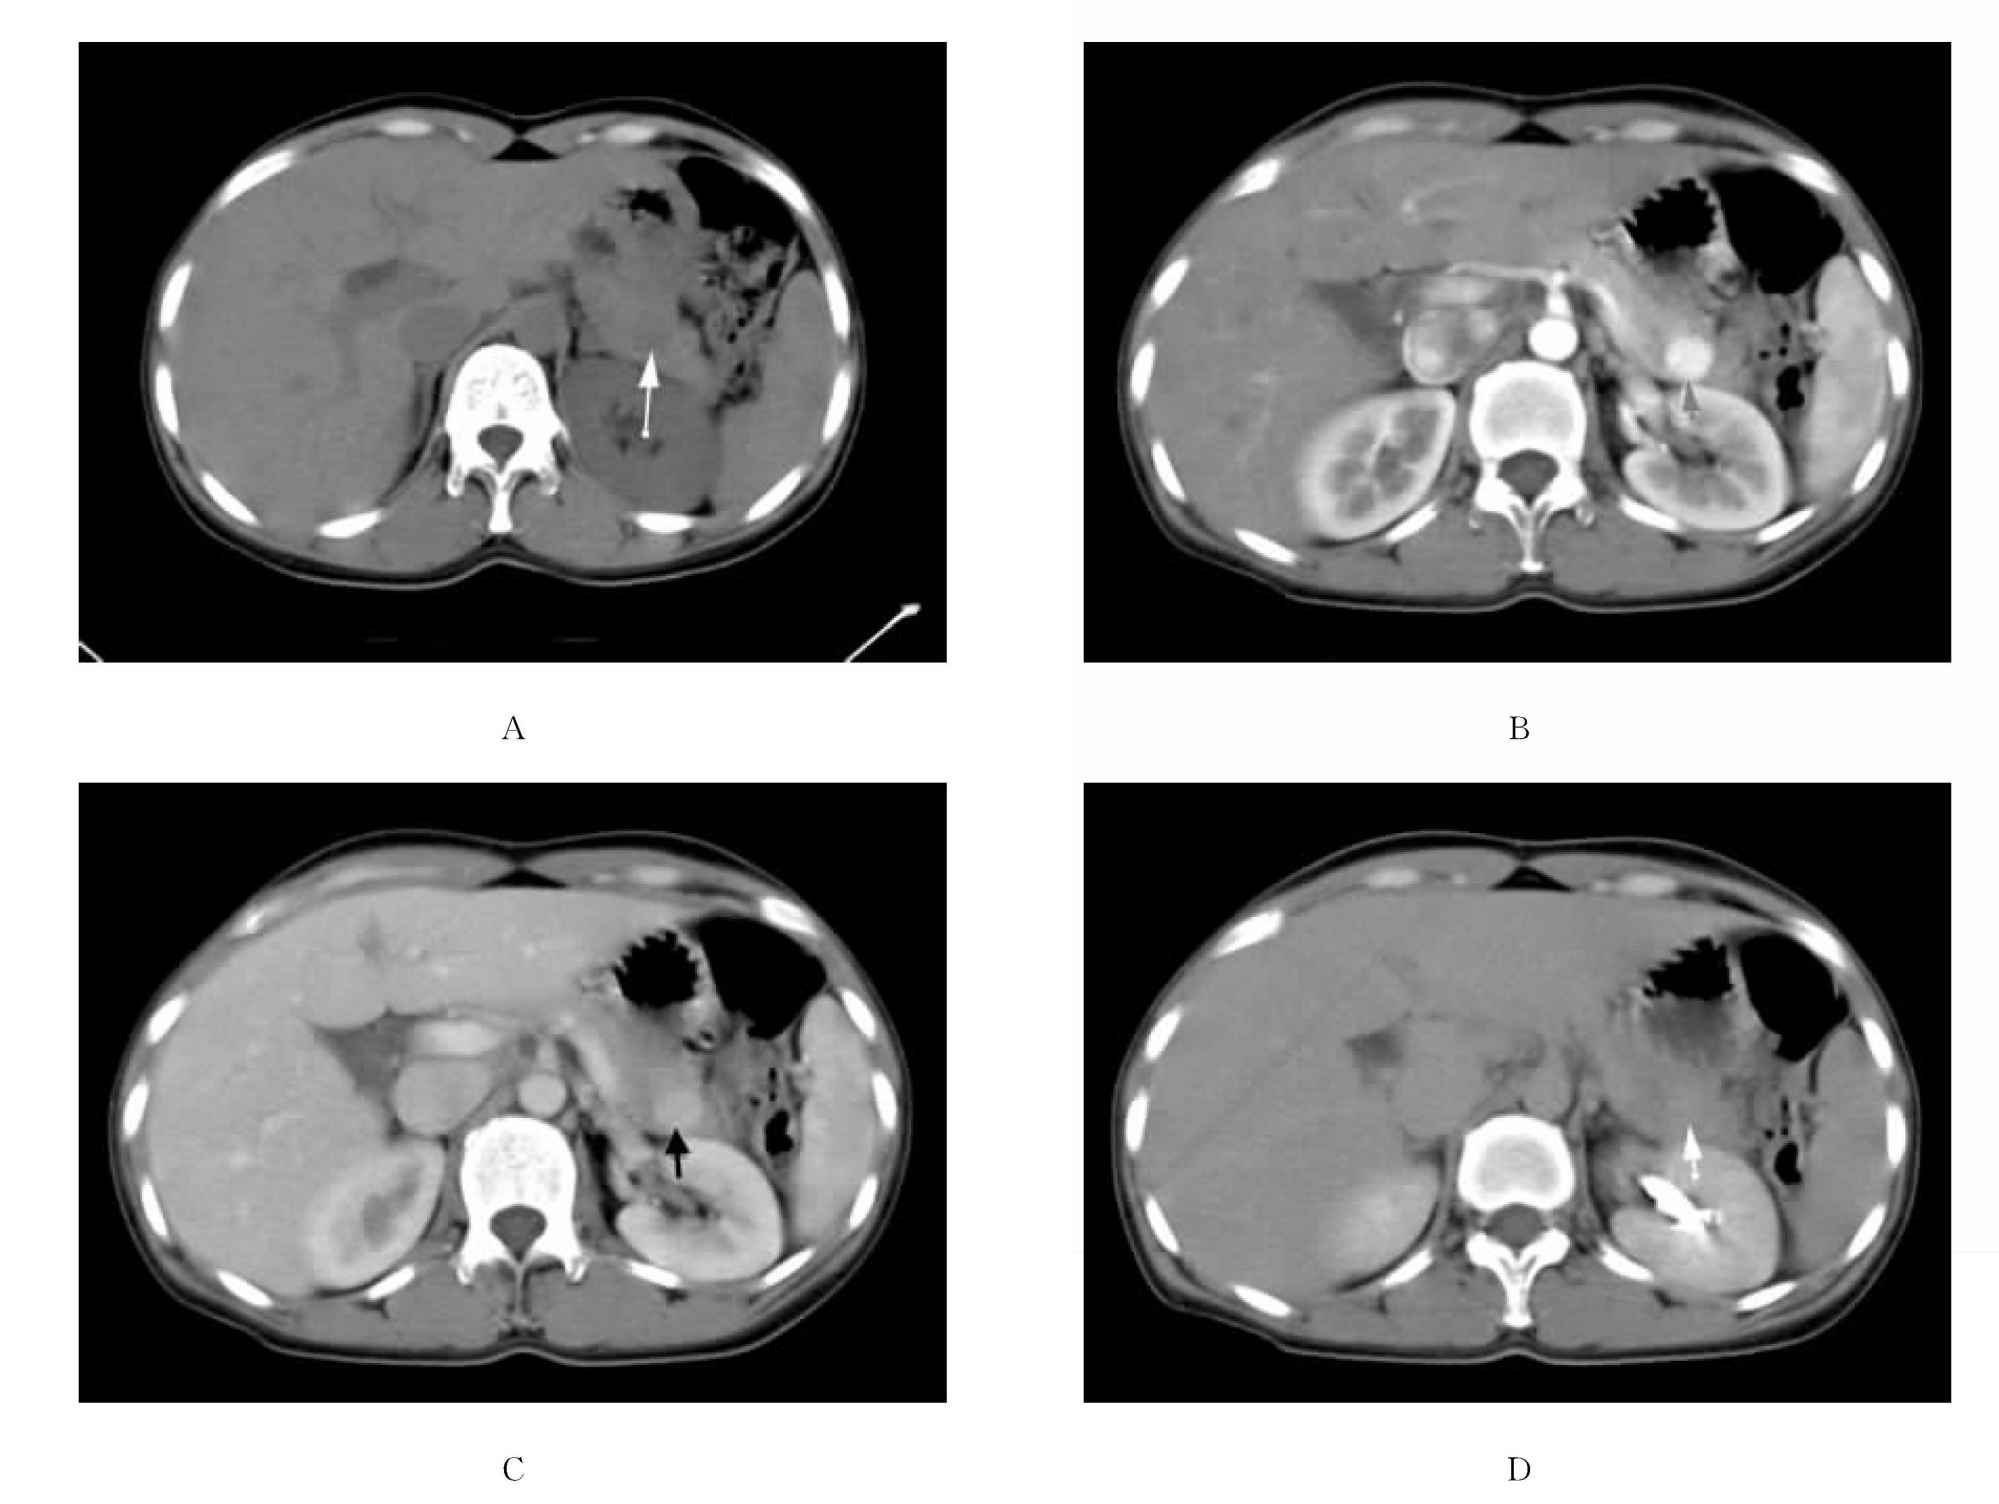
\includegraphics[width=.7\textwidth,height=\textheight,keepaspectratio]{./images/Image00307.jpg}
 \captionsetup{justification=centering}
 \caption{胰岛素瘤\\{\small 36岁女性,反复晕厥1年余;血糖减低。A~D分别为平扫、动脉期、门静脉期、延迟期(延迟5分钟)扫描。胰尾部有约2.0cm低密度结节,边缘光整,增强扫描动脉期显著强化(增强值约100Hu)、门静脉期略减低,延迟期病灶近等密度}}
 \label{fig13-6}
  \end{figure} 

2.无功能性胰岛细胞瘤:较大的肿块,一般>3cm,有文献报道平均直径10cm左右;多发生于胰体、尾部。约20%出现瘤体内钙化,呈孤立结节状。增强扫描可为均匀或不均匀强化,密度可高于、等于或低于正常胰腺,中心可出现坏死、囊变。恶性变可有胰周淋巴结增大、肝转移等征象。

由于胰岛细胞瘤的良、恶性在病理组织学上很难鉴别,仅靠是否浸润性生长、肿瘤有否转移作出判断,故影像学检查综合分析在良恶性鉴别上有重要作用。

\textbf{【鉴别诊断】}
功能性胰岛细胞瘤体积较小、富血供强化的特点,结合临床及实验室检查不难做出正确诊断。而无功能性胰岛细胞瘤需与下列疾病鉴别:

1.胰腺癌:①无功能性胰岛细胞瘤较大,直径常可>10cm;而胰腺癌肿块相对较小;②前者为多血管性,增强后肿块密度一般高于胰腺;而后者则相反;③前者瘤体钙化率高(20%~25%);后者较少(2%);④前者一般不出现胰腺后方动脉周围的侵犯,如腹腔动脉干及肠系膜上动脉等;而后者常见;⑤前者肝内转移灶也表现为富血供;而后者相反。

2.胰腺囊腺癌:可呈圆形、囊性低密度肿块,常为多房性,也可为单房性;多有囊壁,且囊壁厚薄不一,并可见壁结节,较为特征。囊内可见分隔。增强后囊壁、壁结节及囊内分隔有强化,据此多可与无功能性胰岛细胞瘤鉴别。

3.胰头慢性炎症合并假囊肿或脓肿:可表现为胰头增大伴胰头内囊肿或脓肿。中心可呈圆形均匀低密度,边界光整,与无功能性胰岛细胞瘤可相似。但周围有轻微炎症渗出,脂肪层内可见条索状高密度,有时伴肾筋膜增厚,结合病史可予鉴别。

\subsection{胰腺实性-假乳头状瘤}

本病又称胰腺乳头状囊性肿瘤、囊实性乳头状上皮性肿瘤、实性腺泡细胞瘤、乳头状囊性及实性瘤等。是一种少见的组织来源尚不明确的低度恶性肿瘤。

\textbf{【病理】}
其特点为肿瘤由实性区、假乳头状区及两者过渡区,以不同比例混合而成。假乳头状区肿瘤组织以纤细的纤维血管为中心形成分支状假乳头,其表面细胞呈复层排列;远离血管周围的肿瘤细胞发生退行性变,而表现为不同程度的出血、坏死、液化及囊性变,即形成了CT所见的囊性区。故囊性区由坏死、液化、陈旧性出血所致,但囊变、坏死与瘤体大小无关。肿瘤的实性部分有良好的血管,可以出现钙化。此外,实性与假乳头之间的过渡区,表现为肿瘤组织围绕血管形成假菊形团,大部分肿瘤组织呈网状排列,之间形成血窦,类似海绵状血管瘤(所以门静脉期肿瘤实性部分显著强化)。

\textbf{【临床表现】}
常见于年轻女性,偶发于老年妇女和男性。最常见的症状是上腹部疼痛、不适且夜间加重,少数出现腰背部疼痛及体重减轻等症状,罕见梗阻性黄疸。预后较好。

\textbf{【CT表现】}
病灶可位于胰腺任何部位,肿块大、界限清、有薄包膜。瘤体多位于胰腺边缘处,突出于胰腺轮廓之外,向腹膜腔及腹膜后相对空虚的部位生长。病灶常呈实性与囊性的混杂密度,偶见单纯囊性或实性肿块,故有学者分为囊性成分为主型、囊实性成分均等型和实性成分为主型。囊内充满血凝块或坏死组织,瘤内一般无分隔;偶见瘤体或瘤壁钙化。无论肿瘤发生于胰腺何处,即使巨大胰头肿块,亦罕见胆管、胰管扩张。邻近脏器可受压推移,少有受侵累及征象;无腹膜后、腹膜腔淋巴结肿大。肿瘤多有完整包膜,厚约2~4mm,包膜内壁光滑;增强后包膜明显强化,与胰腺分界清楚,边缘光整。增强扫描动脉期实性部分呈小片状轻度强化,门静脉期呈明显强化。小片状实性部分漂浮在低密度囊性部分中称“浮云征”有一定特征(图\ref{fig13-7})。亦可囊、实性部分相间分布或有壁结节。

\begin{figure}[!htbp]
 \centering
 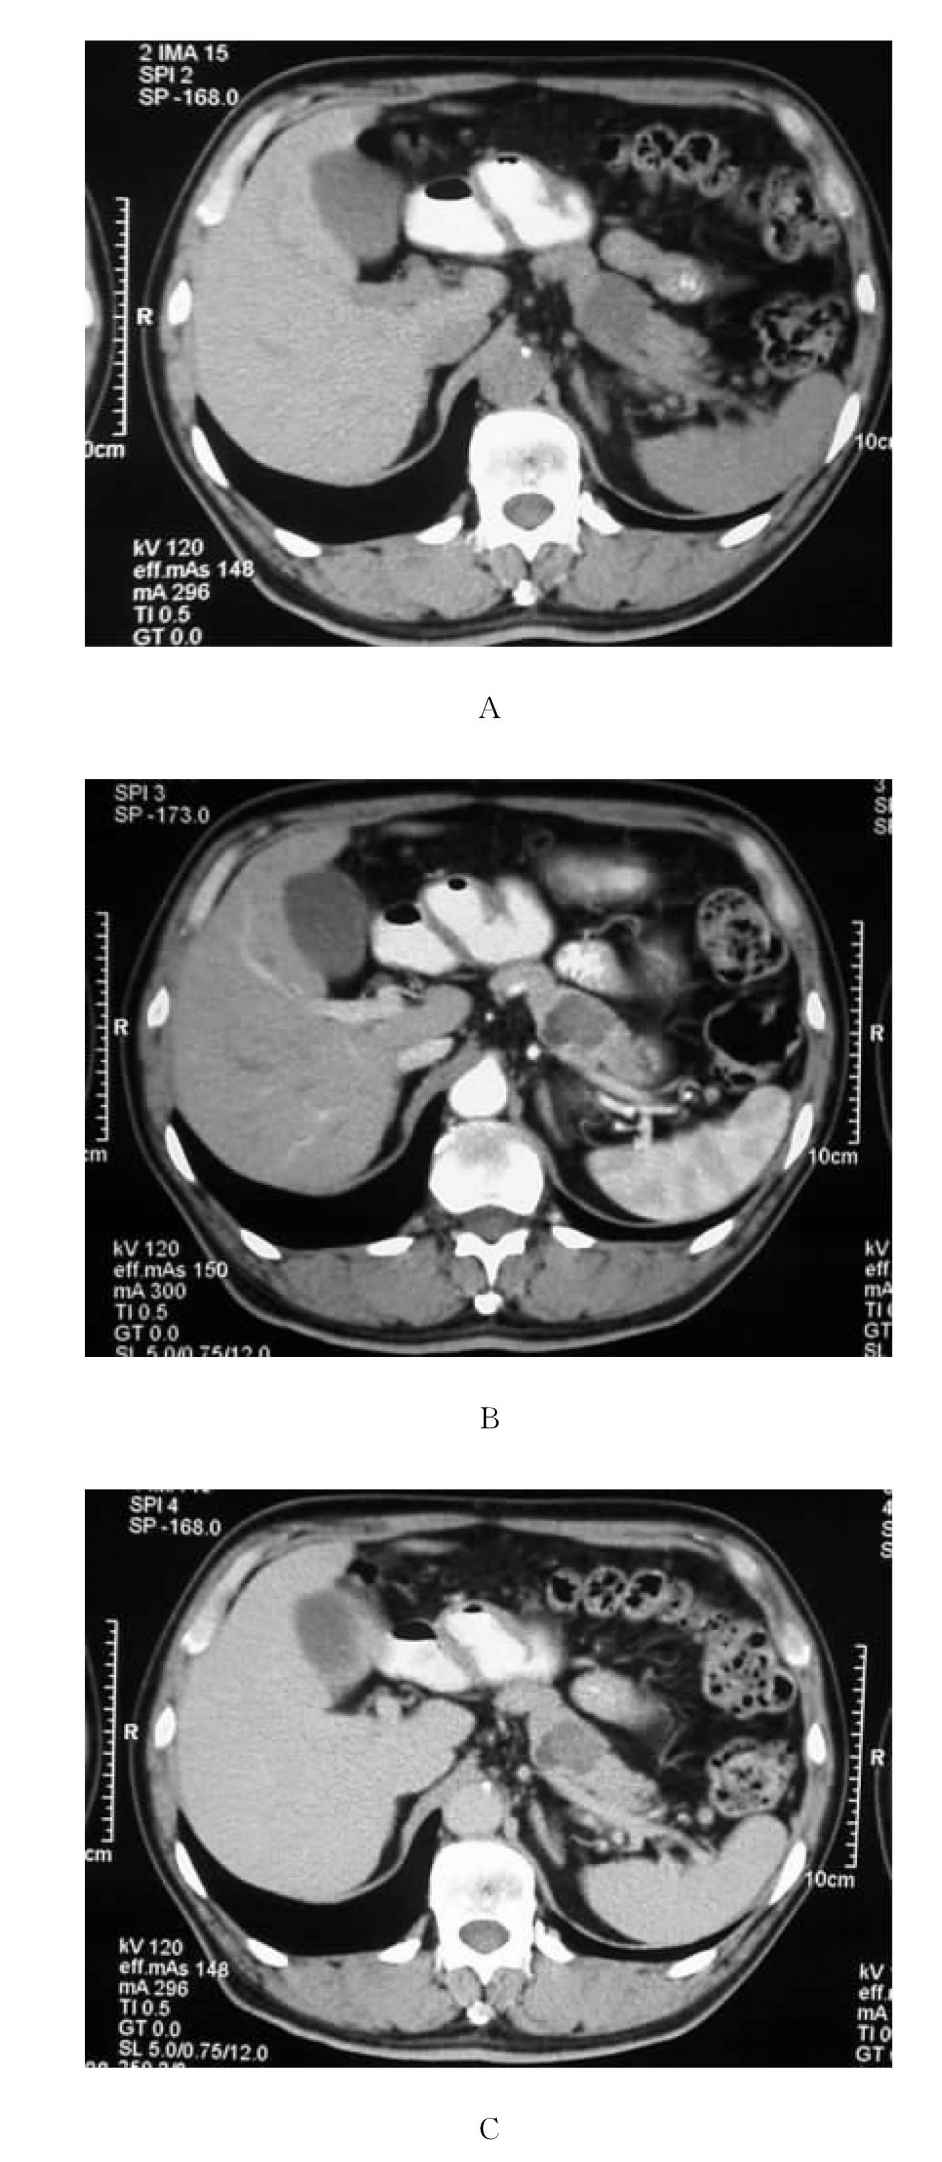
\includegraphics[width=.7\textwidth,height=\textheight,keepaspectratio]{./images/Image00308.jpg}
 \captionsetup{justification=centering}
 \caption{胰腺实性-假乳头状瘤\\{\small A为平扫,胰体部有囊状低密度灶;B为动脉期,C为平衡期,呈小片状强化,小片状实性部分漂浮在低密度囊性部分中即“浮云征”}}
 \label{fig13-7}
  \end{figure} 

本病与囊腺癌CT常难以鉴别。

\subsection{胰腺少见肿瘤}

胰腺少见肿瘤种类甚多,除下述几个外,还有胰腺实性-假乳头状瘤(见上述)、平滑肌瘤和肉瘤、纤维瘤和肉瘤、神经母细胞瘤等,但均无特殊表现,其诊断依靠病理学。

\subsubsection{胰腺多形性癌}

本病即Cubilla分类法中的巨细胞癌,也称为肉瘤样肿瘤。十分罕见,但恶性程度非常高。临床过程极短,极早出现转移灶,预后极差。

\textbf{【病理】}
组织学上由不典型增生的单核细胞、多核巨细胞和梭形细胞构成。

\textbf{【CT表现】}
胰腺实质内可见与一般胰腺癌类似的低密度原发灶。最重要的表现是出现极为广泛的胰周区域淋巴结增大,以致于常误为淋巴瘤。

\subsubsection{胰母细胞瘤}

本病发生于幼儿,属胰腺上皮性肿瘤,又称为婴儿胰腺癌。临床上具有肿瘤局限的特点,预后优于成人胰腺癌。

\textbf{【病理】}
其病理诊断标准是:①具有被膜;②来自腹侧胰头部的肿块;③明显的胰腺器官样结构。

\textbf{【CT表现】}
因具有包膜而肿块边缘清晰;肿块巨大,易坏死、囊变;部分囊壁可见钙化。

\subsubsection{胰腺畸胎瘤}

本病是先天性肿瘤。临床多病史长、症状轻。

\textbf{【病理】}
因其含有内、中、外3个胚层成分,故可有钙化、骨化或脂肪结构。

\textbf{【CT表现】}
多呈囊实混合密度,如见到脂肪、毛发及钙化或骨化影,CT诊断成立。囊性畸胎瘤可见囊壁钙化和囊内脂肪。

\subsubsection{胰腺脂肪瘤或肉瘤}

胰腺脂肪瘤和脂肪肉瘤极罕见。

\textbf{【CT表现】}

1.脂肪瘤:如胰腺肿块为脂肪密度、边缘清楚,则脂肪瘤诊断明确。

2.脂肪肉瘤:如胰腺肿块为脂肪与软组织的混杂密度、边缘模糊,同时见到局部结构受侵或远处转移,则考虑脂肪肉瘤可能。

\subsubsection{胰腺淋巴瘤}

本病占所有胰腺肿瘤的1.5%,往往是全身性淋巴瘤脏器受累的一部分。全身性淋巴瘤胰腺受累的机会不足1%。

\textbf{【病理】}
淋巴肿瘤细胞侵犯胰腺和胰周。通常有胰周、腹膜后淋巴结增大或脾、肾、硬膜外病灶。

\textbf{【CT表现】}
常呈弥漫性胰腺增大,且肿瘤可引起胰腺炎。平扫增大的胰腺呈均匀一致的稍低密度。局限性者肿块较大,直径多>7cm,密度多均匀,边缘模糊,侵犯胰周脏器及结构。可继发胆管和胰管扩张,但有文献报道胰管阻塞极少见。增强扫描病灶稍有强化。可有胰周、腹膜后淋巴结增大和其他脏器受侵表现。

\subsubsection{胰腺转移瘤}

本病的原发肿瘤有肾细胞癌、支气管肺癌、乳腺癌、软组织肉瘤、结肠癌、黑色素瘤、卵巢癌、前列腺癌、精原细胞癌等。

\textbf{【CT表现】}
国外有资料统计:近80%为单发、少数为多发、偶见弥漫性,肿瘤的分布没有显著性差异。病灶多呈圆形或椭圆形,有一些呈分叶状;大多数肿瘤边缘清楚,但边缘多不连续。增强扫描大多数肿瘤有明显高于胰腺实质的强化部分,但大多为不均匀强化。约1/5的肿瘤显示为完全低密度。有时肿瘤含有囊性成分,个别以囊性为主,偶见钙化(如肾癌、结肠癌)。少数可有胰管甚至胆管梗阻扩张。

\subsubsection{胰腺血管球瘤}

\textbf{【临床表现】}
多见于中老年女性。肿瘤生长缓慢,幼年时无自觉症状,长大时可有隐痛,多为血管球瘤内压增高所致。肿瘤因不含神经而不发生剧痛。

\textbf{【CT表现】}
与肝血管瘤类似,但因富血供有时与胰岛细胞瘤难以鉴别,尤其是恶变成肉瘤则不能与其他恶性肿瘤鉴别。

\subsection{胰腺囊样病变的鉴别诊断}

1.病因:可为炎症性、肿瘤性和先天性。假性囊肿最常见,还可见于胰腺癌囊变、胰腺癌合并囊肿、囊腺瘤、囊腺癌、无功能性胰岛细胞瘤、真性囊肿。罕见的病因有囊性畸胎瘤、胰母细胞瘤、神经鞘瘤、实性-假乳头状瘤、肉瘤、转移瘤、包虫病、脓肿、结核、囊性纤维化等。

2.囊壁及钙化:①薄壁可见于囊肿、囊腺肿瘤或非功能胰岛细胞瘤,少见的有囊性畸胎瘤、神经鞘瘤等。②假性囊肿早期薄、成熟期厚可伴钙化。伴感染时壁厚但无壁结节,周围界限清,多无强化。③囊腺肿瘤多有壁结节(恶性者厚度多>1cm,且囊壁厚薄不均),囊壁和结节可有中度以上强化。可有钙化,且黏液性囊腺瘤(癌)钙化多在外围,而浆液性囊腺瘤的特征是中心点状瘢痕及放射状钙化。但两者钙化发生率均不足50%。④胰岛细胞瘤囊壁也可钙化,且钙化的出现可能随囊变体积的增大而增大。其囊壁可有较明显强化。⑤囊壁的完全环形钙化、偏侧性条状钙化多见于假性囊肿、囊腺瘤等;断续性环形钙化,模糊的斑点、条状钙化多为囊腺癌。⑥胰腺癌坏死囊变,壁厚薄不均,与周围界限不清楚。

3.分隔:有分隔强烈提示肿瘤性病变,尤其是囊腺肿瘤,囊样非功能性胰岛细胞瘤也可有分隔。分隔多强化较明显。恶性者分隔厚薄不一、不规则。

4.数目:若为多个不同部位发生,囊肿可能性大。肿瘤性病变多为单发,但囊腺肿瘤可有多个子囊。

5.胰腺炎征象:病史及其实验室检查有助于胰腺炎合并假性囊肿的诊断,但胰腺炎与胰腺癌可互为因果,应予注意。

6.大小及部位:基本意义不大。

7.周围改变:①良性病变对周围组织以推压为主,可有粘连;②恶性病变可粘连、侵犯周围组织及血管,并可有周围淋巴结增大及远处转移。囊腺瘤和癌、胰岛细胞瘤良恶性的鉴别主要依靠上述表现。

8.性别及年龄:如非功能性胰岛细胞瘤女性多见,且年龄多<30岁。囊腺肿瘤好发于女性,年龄多>50岁。

\protect\hypertarget{text00021.html}{}{}

